% Options for packages loaded elsewhere
\PassOptionsToPackage{unicode}{hyperref}
\PassOptionsToPackage{hyphens}{url}
%
\documentclass[
]{article}
\usepackage{amsmath,amssymb}
\usepackage{iftex}
\ifPDFTeX
  \usepackage[T1]{fontenc}
  \usepackage[utf8]{inputenc}
  \usepackage{textcomp} % provide euro and other symbols
\else % if luatex or xetex
  \usepackage{unicode-math} % this also loads fontspec
  \defaultfontfeatures{Scale=MatchLowercase}
  \defaultfontfeatures[\rmfamily]{Ligatures=TeX,Scale=1}
\fi
\usepackage{lmodern}
\ifPDFTeX\else
  % xetex/luatex font selection
\fi
% Use upquote if available, for straight quotes in verbatim environments
\IfFileExists{upquote.sty}{\usepackage{upquote}}{}
\IfFileExists{microtype.sty}{% use microtype if available
  \usepackage[]{microtype}
  \UseMicrotypeSet[protrusion]{basicmath} % disable protrusion for tt fonts
}{}
\makeatletter
\@ifundefined{KOMAClassName}{% if non-KOMA class
  \IfFileExists{parskip.sty}{%
    \usepackage{parskip}
  }{% else
    \setlength{\parindent}{0pt}
    \setlength{\parskip}{6pt plus 2pt minus 1pt}}
}{% if KOMA class
  \KOMAoptions{parskip=half}}
\makeatother
\usepackage{xcolor}
\usepackage[margin=1in]{geometry}
\usepackage{color}
\usepackage{fancyvrb}
\newcommand{\VerbBar}{|}
\newcommand{\VERB}{\Verb[commandchars=\\\{\}]}
\DefineVerbatimEnvironment{Highlighting}{Verbatim}{commandchars=\\\{\}}
% Add ',fontsize=\small' for more characters per line
\usepackage{framed}
\definecolor{shadecolor}{RGB}{248,248,248}
\newenvironment{Shaded}{\begin{snugshade}}{\end{snugshade}}
\newcommand{\AlertTok}[1]{\textcolor[rgb]{0.94,0.16,0.16}{#1}}
\newcommand{\AnnotationTok}[1]{\textcolor[rgb]{0.56,0.35,0.01}{\textbf{\textit{#1}}}}
\newcommand{\AttributeTok}[1]{\textcolor[rgb]{0.13,0.29,0.53}{#1}}
\newcommand{\BaseNTok}[1]{\textcolor[rgb]{0.00,0.00,0.81}{#1}}
\newcommand{\BuiltInTok}[1]{#1}
\newcommand{\CharTok}[1]{\textcolor[rgb]{0.31,0.60,0.02}{#1}}
\newcommand{\CommentTok}[1]{\textcolor[rgb]{0.56,0.35,0.01}{\textit{#1}}}
\newcommand{\CommentVarTok}[1]{\textcolor[rgb]{0.56,0.35,0.01}{\textbf{\textit{#1}}}}
\newcommand{\ConstantTok}[1]{\textcolor[rgb]{0.56,0.35,0.01}{#1}}
\newcommand{\ControlFlowTok}[1]{\textcolor[rgb]{0.13,0.29,0.53}{\textbf{#1}}}
\newcommand{\DataTypeTok}[1]{\textcolor[rgb]{0.13,0.29,0.53}{#1}}
\newcommand{\DecValTok}[1]{\textcolor[rgb]{0.00,0.00,0.81}{#1}}
\newcommand{\DocumentationTok}[1]{\textcolor[rgb]{0.56,0.35,0.01}{\textbf{\textit{#1}}}}
\newcommand{\ErrorTok}[1]{\textcolor[rgb]{0.64,0.00,0.00}{\textbf{#1}}}
\newcommand{\ExtensionTok}[1]{#1}
\newcommand{\FloatTok}[1]{\textcolor[rgb]{0.00,0.00,0.81}{#1}}
\newcommand{\FunctionTok}[1]{\textcolor[rgb]{0.13,0.29,0.53}{\textbf{#1}}}
\newcommand{\ImportTok}[1]{#1}
\newcommand{\InformationTok}[1]{\textcolor[rgb]{0.56,0.35,0.01}{\textbf{\textit{#1}}}}
\newcommand{\KeywordTok}[1]{\textcolor[rgb]{0.13,0.29,0.53}{\textbf{#1}}}
\newcommand{\NormalTok}[1]{#1}
\newcommand{\OperatorTok}[1]{\textcolor[rgb]{0.81,0.36,0.00}{\textbf{#1}}}
\newcommand{\OtherTok}[1]{\textcolor[rgb]{0.56,0.35,0.01}{#1}}
\newcommand{\PreprocessorTok}[1]{\textcolor[rgb]{0.56,0.35,0.01}{\textit{#1}}}
\newcommand{\RegionMarkerTok}[1]{#1}
\newcommand{\SpecialCharTok}[1]{\textcolor[rgb]{0.81,0.36,0.00}{\textbf{#1}}}
\newcommand{\SpecialStringTok}[1]{\textcolor[rgb]{0.31,0.60,0.02}{#1}}
\newcommand{\StringTok}[1]{\textcolor[rgb]{0.31,0.60,0.02}{#1}}
\newcommand{\VariableTok}[1]{\textcolor[rgb]{0.00,0.00,0.00}{#1}}
\newcommand{\VerbatimStringTok}[1]{\textcolor[rgb]{0.31,0.60,0.02}{#1}}
\newcommand{\WarningTok}[1]{\textcolor[rgb]{0.56,0.35,0.01}{\textbf{\textit{#1}}}}
\usepackage{longtable,booktabs,array}
\usepackage{calc} % for calculating minipage widths
% Correct order of tables after \paragraph or \subparagraph
\usepackage{etoolbox}
\makeatletter
\patchcmd\longtable{\par}{\if@noskipsec\mbox{}\fi\par}{}{}
\makeatother
% Allow footnotes in longtable head/foot
\IfFileExists{footnotehyper.sty}{\usepackage{footnotehyper}}{\usepackage{footnote}}
\makesavenoteenv{longtable}
\usepackage{graphicx}
\makeatletter
\def\maxwidth{\ifdim\Gin@nat@width>\linewidth\linewidth\else\Gin@nat@width\fi}
\def\maxheight{\ifdim\Gin@nat@height>\textheight\textheight\else\Gin@nat@height\fi}
\makeatother
% Scale images if necessary, so that they will not overflow the page
% margins by default, and it is still possible to overwrite the defaults
% using explicit options in \includegraphics[width, height, ...]{}
\setkeys{Gin}{width=\maxwidth,height=\maxheight,keepaspectratio}
% Set default figure placement to htbp
\makeatletter
\def\fps@figure{htbp}
\makeatother
\setlength{\emergencystretch}{3em} % prevent overfull lines
\providecommand{\tightlist}{%
  \setlength{\itemsep}{0pt}\setlength{\parskip}{0pt}}
\setcounter{secnumdepth}{-\maxdimen} % remove section numbering
\usepackage{geometry}
\geometry{a4paper, landscape, margin=1in}
\usepackage{booktabs}
\usepackage{longtable}
\usepackage{array}
\usepackage{multirow}
\usepackage{wrapfig}
\usepackage{float}
\usepackage{colortbl}
\usepackage{pdflscape}
\usepackage{tabu}
\usepackage{threeparttable}
\usepackage{threeparttablex}
\usepackage[normalem]{ulem}
\usepackage{makecell}
\usepackage{xcolor}
\ifLuaTeX
  \usepackage{selnolig}  % disable illegal ligatures
\fi
\usepackage{bookmark}
\IfFileExists{xurl.sty}{\usepackage{xurl}}{} % add URL line breaks if available
\urlstyle{same}
\hypersetup{
  pdftitle={Spotify Data Analysis and Music Recommendation System},
  pdfauthor={Mitansh Maheshwari},
  hidelinks,
  pdfcreator={LaTeX via pandoc}}

\title{Spotify Data Analysis and Music Recommendation System}
\author{Mitansh Maheshwari}
\date{2024-10-25}

\begin{document}
\maketitle

\section{Project Overview}\label{project-overview}

In an age where music streaming has become a predominant mode of
consuming music, understanding user listening habits is crucial for
enhancing user experience and satisfaction. This project focuses on
analyzing Spotify streaming data to develop a music recommendation
system that personalizes music suggestions based on individual user
preferences. By harnessing user listening history and audio feature
data, the project aims to identify patterns in music consumption,
ultimately creating a tailored recommendation engine that enhances the
user's music discovery experience.

\subsubsection{Problem Statement}\label{problem-statement}

As the landscape of music streaming evolves, understanding user behavior
and preferences has become increasingly essential for enhancing user
engagement and satisfaction. Despite the vast amounts of data generated
by listeners on platforms like Spotify, there is a lack of comprehensive
analysis that explores the nuanced relationships between listening
habits, emotional responses, and audio features.

The primary challenges this project aims to address include:

\begin{itemize}
\item
  \textbf{Understanding Listening Patterns}: Users exhibit diverse
  listening behaviors influenced by factors such as time of day, day of
  the week, and personal mood. Identifying and analyzing these patterns
  is crucial for tailoring music experiences to individual preferences.
\item
  \textbf{Correlation with Audio Features}: While audio features like
  danceability, energy, and loudness are known to influence user
  engagement, there is insufficient research on how these attributes
  correlate with users' emotional states and overall listening
  satisfaction.
\item
  \textbf{Enhancing Music Discovery}: Users often struggle to discover
  new music that aligns with their tastes, leading to a potential
  decline in engagement. A deeper understanding of user preferences and
  listening contexts is necessary to improve music recommendation
  systems.
\item
  \textbf{User Retention Insights}: Understanding what drives user
  retention on music streaming platforms is essential for developing
  strategies that keep users engaged and satisfied. Identifying key
  factors that contribute to prolonged usage can inform platform
  improvements and content recommendations.
\end{itemize}

By addressing these challenges, this project seeks to provide valuable
insights into user behavior, enhance music discovery through
personalized recommendations, and ultimately improve user satisfaction
and retention on the Spotify platform.

\subsubsection{Purpose}\label{purpose}

The primary purpose of this project is to conduct a comprehensive
analysis of music listening behaviors and patterns among users. By
leveraging extensive streaming data, this project aims to achieve the
following objectives:

\begin{enumerate}
\def\labelenumi{\arabic{enumi}.}
\item
  \textbf{In-depth Analysis of Listening Behavior}: Explore and analyze
  various factors influencing how users interact with music on the
  Spotify platform. This includes examining trends in listening habits
  over time, identifying the impact of different audio features (such as
  danceability, energy, and loudness), and understanding the role of
  contextual elements like time of day and day of the week in shaping
  user preferences.
\item
  \textbf{Enhancing Music Discovery}: Utilize insights gained from the
  data analysis to facilitate personalized music recommendations. By
  understanding user engagement patterns and preferences, the project
  will provide tailored suggestions that help users discover new tracks
  and artists aligned with their tastes, thereby enriching their overall
  music experience.
\item
  \textbf{Informing User Engagement Strategies}: By analyzing listening
  trends and user interactions, the project aims to derive actionable
  insights that can enhance user engagement. Understanding what drives
  user retention and satisfaction will allow for more effective
  marketing strategies and improvements to the Spotify platform,
  ultimately leading to a more enjoyable listening experience for users.
\item
  \textbf{Developing a Recommendation System}: As a secondary goal, this
  project will also focus on creating a recommendation system that
  suggests songs based on a user's mood and listening history. While
  this is a smaller component of the overall project, it aims to
  personalize the user experience further by adapting recommendations to
  individual preferences.
\end{enumerate}

\subsubsection{Objective}\label{objective}

The objectives of this project are designed to guide the analysis of
music listening behaviors and inform the development of personalized
experiences for users. Specifically, we aim to:

\begin{enumerate}
\def\labelenumi{\arabic{enumi}.}
\item
  \textbf{Examine User Listening Patterns}: Analyze streaming data to
  identify trends and variations in user listening habits over time,
  focusing on factors such as time of day, day of the week, and genre
  preferences.
\item
  \textbf{Investigate Audio Features}: Explore how specific audio
  characteristics---such as danceability, energy, valence, loudness, and
  instrumentalness---affect user engagement and listening time. This
  will help to understand the attributes that contribute to users'
  enjoyment of music.
\item
  \textbf{Analyze Mood Correlations}: Assess how users' moods correlate
  with their music choices. By examining the emotional resonance of
  songs, we can identify patterns that can be leveraged to enhance music
  discovery.
\item
  \textbf{Identify High-Engagement Tracks and Artists}: Determine which
  tracks and artists exhibit the highest levels of user engagement.
  Understanding these metrics will provide valuable insights into
  popular content and user preferences.
\item
  \textbf{Develop a Mood-Based Recommendation System}: Create a
  recommendation system that suggests songs based on a user's mood and
  listening history, thereby improving music discovery and enhancing the
  overall user experience.
\item
  \textbf{Evaluate User Retention Factors}: Investigate the factors
  contributing to user retention based on their listening habits. By
  identifying key elements that keep users engaged with the platform, we
  can inform strategies for improving user satisfaction.
\end{enumerate}

\subsubsection{Methodology}\label{methodology}

\begin{enumerate}
\def\labelenumi{\arabic{enumi}.}
\item
  \textbf{Data Collection}: The data for this project was collected from
  Spotify through the Spotify API. I requested my listening history for
  the past year, which included key fields such as \texttt{endTime},
  \texttt{artistName}, \texttt{trackName}, and \texttt{msPlayed}.
  Additionally, audio features like \texttt{danceability},
  \texttt{energy}, \texttt{valence}, \texttt{loudness}, and
  \texttt{instrumentalness} were obtained using the Spotify API to
  enrich the analysis.
\item
  \textbf{Data Wrangling}: The collected data underwent a rigorous
  cleaning and wrangling process to ensure its quality and usability.
  This involved handling missing values by imputing them with mean
  values, ensuring appropriate data types for each variable, and
  filtering out irrelevant entries. The data was then combined into a
  unified dataset, which serves as the foundation for further analysis.
\item
  \textbf{Feature Engineering}: To gain deeper insights into listening
  habits, several new features were engineered from the dataset. This
  included extracting the day of the week, categorizing the time of day
  into periods, and grouping consecutive listening events into sessions.
  Additionally, a listener classification system was developed to
  identify users as Super Listeners, Moderate Listeners, Light
  Listeners, and Occasional Listeners based on their streaming
  frequency.
\item
  \textbf{Data Analysis}: The analysis was conducted using statistical
  methods and visualizations to uncover patterns in listening behavior.
  The relationships between different variables, such as audio features
  and user engagement, were explored to answer key research questions.
  The insights gained from this analysis aimed to inform the development
  of personalized music recommendations.
\item
  \textbf{Visualization and Reporting}: Visualizations were created to
  present the findings from the data analysis in an easily interpretable
  format. These included graphs and charts that illustrate user
  listening patterns, engagement metrics, and correlations between audio
  features and user behavior. The reporting process aimed to communicate
  the insights effectively, providing a comprehensive overview of the
  project findings and their implications for music discovery.
\item
  \textbf{Recommendation System Development}: a recommendation system
  was designed to suggest tracks based on user preferences. This system
  utilized the insights from the data analysis phase to provide tailored
  recommendations that align with users' musical tastes and moods.
\end{enumerate}

\subsubsection{Conclusion}\label{conclusion}

In summary, this project aims to provide a comprehensive analysis of
music listening behaviors by leveraging Spotify's rich dataset. By
examining user preferences and engagement patterns, we seek to uncover
valuable insights that can enhance the music discovery experience for
users. The methodology outlined above lays the groundwork for
understanding the intricate relationships between various factors
influencing listening habits, ultimately informing the development of a
recommendation system tailored to individual user needs. As we move
forward, the findings from this analysis will contribute to a deeper
understanding of how music impacts our daily lives and how personalized
recommendations can foster a more engaging listening experience.

\begin{center}\rule{0.5\linewidth}{0.5pt}\end{center}

\subsection{Part 1: Data Source and
Collection}\label{part-1-data-source-and-collection}

The dataset utilized in this analysis is derived from Spotify's
streaming history, which captures user listening behaviors over time.
The data was personally requested from Spotify and is provided in two
separate JSON files. Below is a detailed description of the data source,
how it was collected, and the structure of the data files.

\subsubsection{Source of the Data}\label{source-of-the-data}

The primary source of the data is Spotify, a widely used music streaming
service that offers users access to millions of tracks, albums, and
playlists. Spotify allows users to track their listening history, which
includes essential details about the songs they have played, the artists
they have listened to, and the duration of each listening session.

\subsubsection{Data Collection Method}\label{data-collection-method}

To gather the necessary data, I submitted a request through the Spotify
website for my personal listening history. The data arrived within a
week and contains the following key attributes:

\begin{enumerate}
\def\labelenumi{\arabic{enumi}.}
\tightlist
\item
  \textbf{Received Data}:

  \begin{itemize}
  \tightlist
  \item
    The JSON files contain the following attributes for each listening
    event:

    \begin{itemize}
    \tightlist
    \item
      endTime
    \item
      artistName
    \item
      trackName
    \item
      msPlayed
    \end{itemize}
  \end{itemize}
\item
  \textbf{Requested Audio Features:}:

  \begin{itemize}
  \tightlist
  \item
    In addition to the basic listening history data, I utilized the
    Spotify API to request specific audio features for each track. These
    features provide deeper insights into the characteristics of the
    music and include:

    \begin{itemize}
    \tightlist
    \item
      Danceability
    \item
      Energy
    \item
      Valence
    \item
      Loudness
    \item
      Instrumentalness
    \end{itemize}
  \end{itemize}
\end{enumerate}

This dataset, derived from both direct requests to Spotify and the
Spotify API, allows for a comprehensive examination of user listening
history and music characteristics. The rich structure of the data makes
it a valuable resource for building recommendation systems and
understanding user engagement patterns within the Spotify ecosystem.

\subsection{Part 2: Data
Cleaning/Wrangling}\label{part-2-data-cleaningwrangling}

In this section, we focus on the crucial task of data cleaning and
wrangling to prepare the dataset for analysis. This process ensures the
data's quality and consistency, allowing for accurate insights to be
drawn from it. The data cleaning and wrangling were carried out in three
key steps:

\subsubsection{Step 1: Combining Streaming History Data from Multiple
Sources}\label{step-1-combining-streaming-history-data-from-multiple-sources}

In order to analyze listening habits and build a music recommendation
system, it's essential to have a comprehensive dataset. The data used in
this project comes from two separate JSON files (Spotify limits the
amount of streams per file), each containing records of tracks played
over different periods. To ensure seamless analysis, we need to combine
these files into a single dataset.

In this step, we will:

\begin{itemize}
\tightlist
\item
  Read the two JSON files containing streaming history.
\item
  Combine the datasets into a unified structure.
\item
  Save the combined dataset as a new JSON file for further analysis.
\item
  Convert the JSON file to CSV as per Project 1 Requirements.
\end{itemize}

This approach simplifies the data processing workflow and ensures that
we have all relevant information in one place.

\begin{Shaded}
\begin{Highlighting}[]
\CommentTok{\# Load necessary libraries without startup messages}
\FunctionTok{suppressPackageStartupMessages}\NormalTok{(\{}
  \FunctionTok{library}\NormalTok{(jsonlite)}
  \FunctionTok{library}\NormalTok{(dplyr)}
  \FunctionTok{library}\NormalTok{(rmarkdown)}
\NormalTok{\})}

\CommentTok{\# Function to read JSON file and return as a list}
\NormalTok{read\_json\_file }\OtherTok{\textless{}{-}} \ControlFlowTok{function}\NormalTok{(file\_path) \{}
  \FunctionTok{fromJSON}\NormalTok{(file\_path)}
\NormalTok{\}}

\CommentTok{\# Read the two JSON files}
\NormalTok{data\_0 }\OtherTok{\textless{}{-}} \FunctionTok{read\_json\_file}\NormalTok{(}\StringTok{"StreamingHistory\_music\_0.json"}\NormalTok{)}
\NormalTok{data\_1 }\OtherTok{\textless{}{-}} \FunctionTok{read\_json\_file}\NormalTok{(}\StringTok{"StreamingHistory\_music\_1.json"}\NormalTok{)}

\CommentTok{\# Combine the two datasets}
\NormalTok{combined\_data }\OtherTok{\textless{}{-}} \FunctionTok{rbind}\NormalTok{(data\_0, data\_1)}

\CommentTok{\# Write the combined data to a CSV file}
\FunctionTok{write.csv}\NormalTok{(combined\_data, }\AttributeTok{file =} \StringTok{"combined\_data.csv"}\NormalTok{, }\AttributeTok{row.names =} \ConstantTok{FALSE}\NormalTok{)}

\CommentTok{\# Display the first 5 rows of the combined data}
\FunctionTok{head}\NormalTok{(combined\_data, }\DecValTok{5}\NormalTok{)}
\end{Highlighting}
\end{Shaded}

\begin{verbatim}
##            endTime   artistName                          trackName msPlayed
## 1 2023-10-11 23:26 Taylor Swift                      New Romantics   198489
## 2 2023-10-12 00:49 Taylor Swift                      New Romantics    31864
## 3 2023-10-12 00:54 Taylor Swift The Story Of Us (Taylor's Version)   267653
## 4 2023-10-12 00:58 Taylor Swift                           End Game   244826
## 5 2023-10-12 00:59 Taylor Swift         All You Had To Do Was Stay    34933
##   danceability energy valence loudness instrumentalness
## 1        0.653  0.848   0.724   -5.936         4.24e-06
## 2        0.653  0.848   0.724   -5.936         4.24e-06
## 3        0.516  0.784   0.552   -2.636         0.00e+00
## 4        0.649  0.589   0.151   -6.237         0.00e+00
## 5        0.589  0.713   0.540   -5.614         0.00e+00
\end{verbatim}

\subsubsection{Step 2: Data Cleaning
Process}\label{step-2-data-cleaning-process}

In this step, we will clean the combined dataset to ensure its quality
and usability for analysis. This process involves several key actions:

\begin{enumerate}
\def\labelenumi{\arabic{enumi}.}
\item
  \textbf{Handling Missing Values}: We will impute missing values in the
  columns for danceability, energy, valence, loudness, and
  instrumentalness using the mean of their respective columns. This will
  help maintain the integrity of our dataset.
\item
  \textbf{Ensuring Appropriate Data Types}: We will convert the
  \texttt{endTime} column to a proper date-time format and ensure that
  \texttt{msPlayed} is treated as a numeric value.
\item
  \textbf{Filtering Irrelevant Rows}: We will filter out tracks that
  were played for less than a specified duration (e.g., 10 seconds) to
  focus on meaningful listening experiences.
\end{enumerate}

After executing these steps, we will display the first five rows of the
cleaned dataset to confirm the cleaning process's effectiveness.

\begin{Shaded}
\begin{Highlighting}[]
\CommentTok{\# Load necessary libraries}
\FunctionTok{library}\NormalTok{(dplyr)}

\CommentTok{\# Step 2: Read the combined data from the CSV}
\NormalTok{combined\_data }\OtherTok{\textless{}{-}} \FunctionTok{read.csv}\NormalTok{(}\StringTok{"combined\_data.csv"}\NormalTok{)}

\CommentTok{\# Data Cleaning Process}

\CommentTok{\# 1. Handle Missing Values by imputing with the mean}
\NormalTok{combined\_data}\SpecialCharTok{$}\NormalTok{danceability[}\FunctionTok{is.na}\NormalTok{(combined\_data}\SpecialCharTok{$}\NormalTok{danceability)] }\OtherTok{\textless{}{-}} \FunctionTok{mean}\NormalTok{(combined\_data}\SpecialCharTok{$}\NormalTok{danceability, }\AttributeTok{na.rm =} \ConstantTok{TRUE}\NormalTok{)}
\NormalTok{combined\_data}\SpecialCharTok{$}\NormalTok{energy[}\FunctionTok{is.na}\NormalTok{(combined\_data}\SpecialCharTok{$}\NormalTok{energy)] }\OtherTok{\textless{}{-}} \FunctionTok{mean}\NormalTok{(combined\_data}\SpecialCharTok{$}\NormalTok{energy, }\AttributeTok{na.rm =} \ConstantTok{TRUE}\NormalTok{)}
\NormalTok{combined\_data}\SpecialCharTok{$}\NormalTok{valence[}\FunctionTok{is.na}\NormalTok{(combined\_data}\SpecialCharTok{$}\NormalTok{valence)] }\OtherTok{\textless{}{-}} \FunctionTok{mean}\NormalTok{(combined\_data}\SpecialCharTok{$}\NormalTok{valence, }\AttributeTok{na.rm =} \ConstantTok{TRUE}\NormalTok{)}
\NormalTok{combined\_data}\SpecialCharTok{$}\NormalTok{loudness[}\FunctionTok{is.na}\NormalTok{(combined\_data}\SpecialCharTok{$}\NormalTok{loudness)] }\OtherTok{\textless{}{-}} \FunctionTok{mean}\NormalTok{(combined\_data}\SpecialCharTok{$}\NormalTok{loudness, }\AttributeTok{na.rm =} \ConstantTok{TRUE}\NormalTok{)}
\NormalTok{combined\_data}\SpecialCharTok{$}\NormalTok{instrumentalness[}\FunctionTok{is.na}\NormalTok{(combined\_data}\SpecialCharTok{$}\NormalTok{instrumentalness)] }\OtherTok{\textless{}{-}} \FunctionTok{mean}\NormalTok{(combined\_data}\SpecialCharTok{$}\NormalTok{instrumentalness, }\AttributeTok{na.rm =} \ConstantTok{TRUE}\NormalTok{)}

\CommentTok{\# 2. Ensure appropriate data types}
\NormalTok{combined\_data}\SpecialCharTok{$}\NormalTok{endTime }\OtherTok{\textless{}{-}} \FunctionTok{as.POSIXct}\NormalTok{(combined\_data}\SpecialCharTok{$}\NormalTok{endTime)}
\NormalTok{combined\_data}\SpecialCharTok{$}\NormalTok{msPlayed }\OtherTok{\textless{}{-}} \FunctionTok{as.numeric}\NormalTok{(combined\_data}\SpecialCharTok{$}\NormalTok{msPlayed)}

\CommentTok{\# 3. Filter out irrelevant rows (example: keep tracks played for more than 10 seconds)}
\NormalTok{combined\_data }\OtherTok{\textless{}{-}}\NormalTok{ combined\_data }\SpecialCharTok{\%\textgreater{}\%} \FunctionTok{filter}\NormalTok{(msPlayed }\SpecialCharTok{\textgreater{}} \DecValTok{10000}\NormalTok{)}

\FunctionTok{head}\NormalTok{(combined\_data, }\DecValTok{5}\NormalTok{)}
\end{Highlighting}
\end{Shaded}

\begin{verbatim}
##               endTime   artistName                          trackName msPlayed
## 1 2023-10-11 23:26:00 Taylor Swift                      New Romantics   198489
## 2 2023-10-12 00:49:00 Taylor Swift                      New Romantics    31864
## 3 2023-10-12 00:54:00 Taylor Swift The Story Of Us (Taylor's Version)   267653
## 4 2023-10-12 00:58:00 Taylor Swift                           End Game   244826
## 5 2023-10-12 00:59:00 Taylor Swift         All You Had To Do Was Stay    34933
##   danceability energy valence loudness instrumentalness
## 1        0.653  0.848   0.724   -5.936         4.24e-06
## 2        0.653  0.848   0.724   -5.936         4.24e-06
## 3        0.516  0.784   0.552   -2.636         0.00e+00
## 4        0.649  0.589   0.151   -6.237         0.00e+00
## 5        0.589  0.713   0.540   -5.614         0.00e+00
\end{verbatim}

\subsubsection{Step 3: Feature
Engineering}\label{step-3-feature-engineering}

In this step, we will enhance our dataset by creating new features that
can provide deeper insights into listening habits and preferences.
Feature engineering is a critical process in data analysis and machine
learning, as it can significantly improve the performance of models by
introducing informative attributes. Below are the newly created
variables/features:

\begin{enumerate}
\def\labelenumi{\arabic{enumi}.}
\tightlist
\item
  \textbf{Day of the Week}:

  \begin{itemize}
  \tightlist
  \item
    \textbf{Variable Name}: \texttt{day\_of\_week}
  \item
    \textbf{Description}: This variable extracts the day of the week
    from the \texttt{endTime} column, allowing us to analyze patterns in
    listening behavior based on weekdays versus weekends. By knowing the
    day of the week, we can identify trends in music consumption, such
    as whether users listen more on weekends compared to weekdays.
  \item
    \textbf{Values}: This variable can take on values such as
    ``Monday,'' ``Tuesday,'' ``Wednesday,'' ``Thursday,'' ``Friday,''
    ``Saturday,'' and ``Sunday.''
  \end{itemize}
\item
  \textbf{Time of Day}

  \begin{itemize}
  \tightlist
  \item
    \textbf{Variable Name:} \texttt{time\_of\_day}
  \item
    \textbf{Description:} This variable categorizes the listening times
    into distinct periods of the day: Night, Morning, Afternoon,
    Evening, and Late Night. Understanding when users listen to music
    can help in creating personalized recommendations based on peak
    listening times.
  \item
    \textbf{Values:}

    \begin{itemize}
    \tightlist
    \item
      Night: From 12:00 AM to 5:00 AM
    \item
      Morning: From 6:00 AM to 11:00 AM
    \item
      Afternoon: From 12:00 PM to 5:00 PM
    \item
      Evening: From 6:00 PM to 9:00 PM
    \item
      Late Night: From 10:00 PM to 11:59 PM
    \end{itemize}
  \end{itemize}
\item
  \textbf{Listening Session ID}:

  \begin{itemize}
  \tightlist
  \item
    \textbf{Variable Name}: \texttt{session\_id}
  \item
    \textbf{Description}: This variable groups consecutive listening
    events into sessions based on a defined time window (in this case,
    30 minutes). By identifying listening sessions, we can better
    understand user engagement and the depth of their listening
    experiences. This feature helps to analyze how users consume music
    over a period rather than individual tracks.
  \item
    \textbf{Values}: Each session will be represented by a unique ID,
    with consecutive events grouped together. For example, if a user
    listens to several songs in one session, they will have the same
    session\_id until there is a break of more than 30 minutes.
  \end{itemize}
\item
  \textbf{Listener Categories}

  \begin{itemize}
  \tightlist
  \item
    \textbf{Variable Name:} \texttt{listener\_category}
  \item
    \textbf{Description:} This variable categorizes artists based on
    their play counts into four distinct groups: Super Listeners,
    Moderate Listeners, Light Listeners, and Occasional Listeners. This
    categorization helps to identify user engagement with different
    artists, providing insights into listening preferences and
    facilitating personalized recommendations.
  \item
    \textbf{Values:}

    \begin{itemize}
    \tightlist
    \item
      \textbf{Super Listeners:} More than 100 streams, indicating a high
      level of engagement and strong preference for the artist.
    \item
      \textbf{Moderate Listeners:} Between 50 and 100 streams,
      reflecting considerable interest and occasional engagement with
      the artist.
    \item
      \textbf{Light Listeners:} Between 10 and 50 streams, suggesting
      that the artist has some appeal but is not a primary choice for
      the listener.
    \item
      \textbf{Occasional Listeners:} Fewer than 10 streams, indicating
      minimal engagement with the artist, possibly only sampled once or
      twice.
    \end{itemize}
  \end{itemize}
\end{enumerate}

\begin{Shaded}
\begin{Highlighting}[]
\CommentTok{\# Feature Engineering Implementation}
\CommentTok{\# 1. Day of the Week}
\NormalTok{combined\_data}\SpecialCharTok{$}\NormalTok{day\_of\_week }\OtherTok{\textless{}{-}} \FunctionTok{weekdays}\NormalTok{(combined\_data}\SpecialCharTok{$}\NormalTok{endTime)}

\CommentTok{\# 2. Time of Day}
\NormalTok{combined\_data}\SpecialCharTok{$}\NormalTok{time\_of\_day }\OtherTok{\textless{}{-}} \FunctionTok{cut}\NormalTok{(}\FunctionTok{as.numeric}\NormalTok{(}\FunctionTok{format}\NormalTok{(combined\_data}\SpecialCharTok{$}\NormalTok{endTime, }\StringTok{"\%H"}\NormalTok{)),}
                                  \AttributeTok{breaks =} \FunctionTok{c}\NormalTok{(}\SpecialCharTok{{-}}\DecValTok{1}\NormalTok{, }\DecValTok{5}\NormalTok{, }\DecValTok{11}\NormalTok{, }\DecValTok{17}\NormalTok{, }\DecValTok{21}\NormalTok{, }\DecValTok{24}\NormalTok{),}
                                  \AttributeTok{labels =} \FunctionTok{c}\NormalTok{(}\StringTok{"Night"}\NormalTok{, }\StringTok{"Morning"}\NormalTok{, }\StringTok{"Afternoon"}\NormalTok{, }\StringTok{"Evening"}\NormalTok{, }\StringTok{"LateNight"}\NormalTok{),}
                                  \AttributeTok{right =} \ConstantTok{TRUE}\NormalTok{)}

\CommentTok{\# 3. Listening Session ID}
\NormalTok{combined\_data }\OtherTok{\textless{}{-}}\NormalTok{ combined\_data }\SpecialCharTok{\%\textgreater{}\%}
  \FunctionTok{arrange}\NormalTok{(endTime) }\SpecialCharTok{\%\textgreater{}\%}
  \FunctionTok{mutate}\NormalTok{(}\AttributeTok{session\_id =} \FunctionTok{cumsum}\NormalTok{(}\FunctionTok{c}\NormalTok{(}\DecValTok{1}\NormalTok{, }\FunctionTok{diff}\NormalTok{(endTime) }\SpecialCharTok{\textgreater{}} \DecValTok{1800}\NormalTok{)))}

\CommentTok{\# 4. Listener Categories}
\NormalTok{artist\_play\_counts }\OtherTok{\textless{}{-}}\NormalTok{ combined\_data }\SpecialCharTok{\%\textgreater{}\%}
  \FunctionTok{group\_by}\NormalTok{(artistName) }\SpecialCharTok{\%\textgreater{}\%}
  \FunctionTok{summarise}\NormalTok{(}\AttributeTok{play\_count =} \FunctionTok{n}\NormalTok{()) }\SpecialCharTok{\%\textgreater{}\%}
  \FunctionTok{ungroup}\NormalTok{()}

\CommentTok{\# Categorize listeners based on play counts}
\NormalTok{artist\_play\_counts }\OtherTok{\textless{}{-}}\NormalTok{ artist\_play\_counts }\SpecialCharTok{\%\textgreater{}\%}
  \FunctionTok{mutate}\NormalTok{(}\AttributeTok{listener\_category =} \FunctionTok{case\_when}\NormalTok{(}
\NormalTok{    play\_count }\SpecialCharTok{\textgreater{}} \DecValTok{100} \SpecialCharTok{\textasciitilde{}} \StringTok{"Super Listeners"}\NormalTok{,}
\NormalTok{    play\_count }\SpecialCharTok{\textgreater{}=} \DecValTok{50} \SpecialCharTok{\&}\NormalTok{ play\_count }\SpecialCharTok{\textless{}=} \DecValTok{100} \SpecialCharTok{\textasciitilde{}} \StringTok{"Moderate Listeners"}\NormalTok{,}
\NormalTok{    play\_count }\SpecialCharTok{\textgreater{}=} \DecValTok{10} \SpecialCharTok{\&}\NormalTok{ play\_count }\SpecialCharTok{\textless{}} \DecValTok{50} \SpecialCharTok{\textasciitilde{}} \StringTok{"Light Listeners"}\NormalTok{,}
\NormalTok{    play\_count }\SpecialCharTok{\textless{}} \DecValTok{10} \SpecialCharTok{\textasciitilde{}} \StringTok{"Occasional Listeners"}
\NormalTok{  ))}

\CommentTok{\# Join the listener category back to the combined data}
\NormalTok{combined\_data }\OtherTok{\textless{}{-}}\NormalTok{ combined\_data }\SpecialCharTok{\%\textgreater{}\%}
  \FunctionTok{left\_join}\NormalTok{(}\FunctionTok{select}\NormalTok{(artist\_play\_counts, artistName, listener\_category), }\AttributeTok{by =} \StringTok{"artistName"}\NormalTok{)}

\CommentTok{\# Display the updated dataset}
\FunctionTok{head}\NormalTok{(combined\_data, }\DecValTok{5}\NormalTok{)}
\end{Highlighting}
\end{Shaded}

\begin{verbatim}
##               endTime   artistName                          trackName msPlayed
## 1 2023-10-11 23:26:00 Taylor Swift                      New Romantics   198489
## 2 2023-10-12 00:49:00 Taylor Swift                      New Romantics    31864
## 3 2023-10-12 00:54:00 Taylor Swift The Story Of Us (Taylor's Version)   267653
## 4 2023-10-12 00:58:00 Taylor Swift                           End Game   244826
## 5 2023-10-12 00:59:00 Taylor Swift         All You Had To Do Was Stay    34933
##   danceability energy valence loudness instrumentalness day_of_week time_of_day
## 1        0.653  0.848   0.724   -5.936         4.24e-06   Wednesday   LateNight
## 2        0.653  0.848   0.724   -5.936         4.24e-06    Thursday       Night
## 3        0.516  0.784   0.552   -2.636         0.00e+00    Thursday       Night
## 4        0.649  0.589   0.151   -6.237         0.00e+00    Thursday       Night
## 5        0.589  0.713   0.540   -5.614         0.00e+00    Thursday       Night
##   session_id listener_category
## 1          1   Super Listeners
## 2          2   Super Listeners
## 3          2   Super Listeners
## 4          2   Super Listeners
## 5          2   Super Listeners
\end{verbatim}

\subsection{Part 3: Exploratory Data
Analysis(EDA)}\label{part-3-exploratory-data-analysiseda}

\subsubsection{Descriptive Statistics}\label{descriptive-statistics}

This section of the analysis focuses on generating descriptive
statistics for key audio features within the Spotify dataset.
Descriptive statistics provide a summary of the central tendency,
dispersion, and shape of the dataset's distribution, which is essential
in exploratory data analysis (EDA) as it helps us understand the basic
properties of the data we are working with.

Descriptive statistics play a crucial role in exploratory data analysis
by providing insights into the characteristics of the data. They help
identify trends, patterns, and anomalies within the dataset, allowing
for informed decision-making in further analysis. Understanding the
central tendency and variability of audio features such as danceability,
energy, valence, loudness, and instrumentalness can lead to better
insights into listener preferences and behavior.

\begin{Shaded}
\begin{Highlighting}[]
\CommentTok{\# Load necessary libraries}
\FunctionTok{library}\NormalTok{(dplyr)}
\FunctionTok{library}\NormalTok{(knitr)}

\CommentTok{\# Assuming the dataset is loaded as \textquotesingle{}combined\_data\textquotesingle{}}

\CommentTok{\# Custom function to calculate mode}
\NormalTok{get\_mode }\OtherTok{\textless{}{-}} \ControlFlowTok{function}\NormalTok{(v) \{}
\NormalTok{  uniq\_v }\OtherTok{\textless{}{-}} \FunctionTok{na.omit}\NormalTok{(}\FunctionTok{unique}\NormalTok{(v))}
\NormalTok{  uniq\_v[}\FunctionTok{which.max}\NormalTok{(}\FunctionTok{tabulate}\NormalTok{(}\FunctionTok{match}\NormalTok{(v, uniq\_v)))]}
\NormalTok{\}}

\CommentTok{\# Calculate mean, median, mode, and standard deviation for key columns}
\NormalTok{summary\_stats }\OtherTok{\textless{}{-}}\NormalTok{ combined\_data }\SpecialCharTok{\%\textgreater{}\%}
  \FunctionTok{summarise}\NormalTok{(}
    \AttributeTok{danceability\_mean =} \FunctionTok{mean}\NormalTok{(danceability, }\AttributeTok{na.rm =} \ConstantTok{TRUE}\NormalTok{),}
    \AttributeTok{danceability\_median =} \FunctionTok{median}\NormalTok{(danceability, }\AttributeTok{na.rm =} \ConstantTok{TRUE}\NormalTok{),}
    \AttributeTok{danceability\_mode =} \FunctionTok{get\_mode}\NormalTok{(danceability),}
    \AttributeTok{danceability\_sd =} \FunctionTok{sd}\NormalTok{(danceability, }\AttributeTok{na.rm =} \ConstantTok{TRUE}\NormalTok{),}
    
    \AttributeTok{energy\_mean =} \FunctionTok{mean}\NormalTok{(energy, }\AttributeTok{na.rm =} \ConstantTok{TRUE}\NormalTok{),}
    \AttributeTok{energy\_median =} \FunctionTok{median}\NormalTok{(energy, }\AttributeTok{na.rm =} \ConstantTok{TRUE}\NormalTok{),}
    \AttributeTok{energy\_mode =} \FunctionTok{get\_mode}\NormalTok{(energy),}
    \AttributeTok{energy\_sd =} \FunctionTok{sd}\NormalTok{(energy, }\AttributeTok{na.rm =} \ConstantTok{TRUE}\NormalTok{),}
    
    \AttributeTok{valence\_mean =} \FunctionTok{mean}\NormalTok{(valence, }\AttributeTok{na.rm =} \ConstantTok{TRUE}\NormalTok{),}
    \AttributeTok{valence\_median =} \FunctionTok{median}\NormalTok{(valence, }\AttributeTok{na.rm =} \ConstantTok{TRUE}\NormalTok{),}
    \AttributeTok{valence\_mode =} \FunctionTok{get\_mode}\NormalTok{(valence),}
    \AttributeTok{valence\_sd =} \FunctionTok{sd}\NormalTok{(valence, }\AttributeTok{na.rm =} \ConstantTok{TRUE}\NormalTok{),}
    
    \AttributeTok{loudness\_mean =} \FunctionTok{mean}\NormalTok{(loudness, }\AttributeTok{na.rm =} \ConstantTok{TRUE}\NormalTok{),}
    \AttributeTok{loudness\_median =} \FunctionTok{median}\NormalTok{(loudness, }\AttributeTok{na.rm =} \ConstantTok{TRUE}\NormalTok{),}
    \AttributeTok{loudness\_mode =} \FunctionTok{get\_mode}\NormalTok{(loudness),}
    \AttributeTok{loudness\_sd =} \FunctionTok{sd}\NormalTok{(loudness, }\AttributeTok{na.rm =} \ConstantTok{TRUE}\NormalTok{),}
    
    \AttributeTok{instrumentalness\_mean =} \FunctionTok{mean}\NormalTok{(instrumentalness, }\AttributeTok{na.rm =} \ConstantTok{TRUE}\NormalTok{),}
    \AttributeTok{instrumentalness\_median =} \FunctionTok{median}\NormalTok{(instrumentalness, }\AttributeTok{na.rm =} \ConstantTok{TRUE}\NormalTok{),}
    \AttributeTok{instrumentalness\_mode =} \FunctionTok{get\_mode}\NormalTok{(instrumentalness),}
    \AttributeTok{instrumentalness\_sd =} \FunctionTok{sd}\NormalTok{(instrumentalness, }\AttributeTok{na.rm =} \ConstantTok{TRUE}\NormalTok{)}
\NormalTok{  )}

\CommentTok{\# Reformat the data to display factors as rows and statistics as columns}
\NormalTok{reformatted\_stats }\OtherTok{\textless{}{-}} \FunctionTok{data.frame}\NormalTok{(}
  \AttributeTok{Factor =} \FunctionTok{c}\NormalTok{(}\StringTok{"Danceability"}\NormalTok{, }\StringTok{"Energy"}\NormalTok{, }\StringTok{"Valence"}\NormalTok{, }\StringTok{"Loudness"}\NormalTok{, }\StringTok{"Instrumentalness"}\NormalTok{),}
  \AttributeTok{Mean =} \FunctionTok{c}\NormalTok{(summary\_stats}\SpecialCharTok{$}\NormalTok{danceability\_mean, summary\_stats}\SpecialCharTok{$}\NormalTok{energy\_mean, summary\_stats}\SpecialCharTok{$}\NormalTok{valence\_mean,}
\NormalTok{           summary\_stats}\SpecialCharTok{$}\NormalTok{loudness\_mean, summary\_stats}\SpecialCharTok{$}\NormalTok{instrumentalness\_mean),}
  \AttributeTok{Median =} \FunctionTok{c}\NormalTok{(summary\_stats}\SpecialCharTok{$}\NormalTok{danceability\_median, summary\_stats}\SpecialCharTok{$}\NormalTok{energy\_median, summary\_stats}\SpecialCharTok{$}\NormalTok{valence\_median,}
\NormalTok{             summary\_stats}\SpecialCharTok{$}\NormalTok{loudness\_median, summary\_stats}\SpecialCharTok{$}\NormalTok{instrumentalness\_median),}
  \AttributeTok{Mode =} \FunctionTok{c}\NormalTok{(summary\_stats}\SpecialCharTok{$}\NormalTok{danceability\_mode, summary\_stats}\SpecialCharTok{$}\NormalTok{energy\_mode, summary\_stats}\SpecialCharTok{$}\NormalTok{valence\_mode,}
\NormalTok{           summary\_stats}\SpecialCharTok{$}\NormalTok{loudness\_mode, summary\_stats}\SpecialCharTok{$}\NormalTok{instrumentalness\_mode),}
  \AttributeTok{SD =} \FunctionTok{c}\NormalTok{(summary\_stats}\SpecialCharTok{$}\NormalTok{danceability\_sd, summary\_stats}\SpecialCharTok{$}\NormalTok{energy\_sd, summary\_stats}\SpecialCharTok{$}\NormalTok{valence\_sd,}
\NormalTok{         summary\_stats}\SpecialCharTok{$}\NormalTok{loudness\_sd, summary\_stats}\SpecialCharTok{$}\NormalTok{instrumentalness\_sd)}
\NormalTok{)}

\CommentTok{\# Display the summary table}
\FunctionTok{kable}\NormalTok{(reformatted\_stats, }\AttributeTok{caption =} \StringTok{"Descriptive Statistics for Key Audio Features"}\NormalTok{)}
\end{Highlighting}
\end{Shaded}

\begin{longtable}[]{@{}lrrrr@{}}
\caption{Descriptive Statistics for Key Audio Features}\tabularnewline
\toprule\noalign{}
Factor & Mean & Median & Mode & SD \\
\midrule\noalign{}
\endfirsthead
\toprule\noalign{}
Factor & Mean & Median & Mode & SD \\
\midrule\noalign{}
\endhead
\bottomrule\noalign{}
\endlastfoot
Danceability & 0.6320172 & 0.632 & 0.632 & 0.1179142 \\
Energy & 0.6711195 & 0.683 & 0.800 & 0.1629690 \\
Valence & 0.5109430 & 0.535 & 0.629 & 0.2280846 \\
Loudness & -6.3737535 & -5.956 & -5.956 & 2.4428684 \\
Instrumentalness & 0.0066805 & 0.000 & 0.000 & 0.0511618 \\
\end{longtable}

\subsubsection{Categorical Analysis}\label{categorical-analysis}

This section focuses on analyzing categorical data within the Spotify
dataset. By examining categories such as listener category, day of the
week, and time of day, we can gain insights into listening behaviors and
preferences across different segments.

Categorical analysis is crucial in exploratory data analysis as it helps
uncover patterns and trends in the data that may not be evident from
numerical analysis alone. By examining how different listener
categories, days of the week, and times of day affect listening
behaviors, we can identify preferences and optimize recommendations or
marketing strategies. Understanding these factors can aid in tailoring
content to better meet the needs of different listener segments,
ultimately enhancing user engagement and satisfaction.

\begin{Shaded}
\begin{Highlighting}[]
\CommentTok{\# Load necessary libraries}
\FunctionTok{library}\NormalTok{(dplyr)}
\FunctionTok{library}\NormalTok{(knitr)}

\CommentTok{\# Check the most common categories in \textquotesingle{}listener\_category\textquotesingle{}}
\CommentTok{\# Count unique artists per listener category}
\NormalTok{categorical\_analysis }\OtherTok{\textless{}{-}}\NormalTok{ combined\_data }\SpecialCharTok{\%\textgreater{}\%}
  \FunctionTok{distinct}\NormalTok{(artistName, listener\_category) }\SpecialCharTok{\%\textgreater{}\%}
  \FunctionTok{group\_by}\NormalTok{(listener\_category) }\SpecialCharTok{\%\textgreater{}\%}
  \FunctionTok{summarise}\NormalTok{(}\AttributeTok{count =} \FunctionTok{n}\NormalTok{()) }\SpecialCharTok{\%\textgreater{}\%}
  \FunctionTok{arrange}\NormalTok{(}\FunctionTok{desc}\NormalTok{(count))}

\CommentTok{\# Display the listener category analysis}
\FunctionTok{kable}\NormalTok{(categorical\_analysis, }\AttributeTok{caption =} \StringTok{"Count of Unique Artists by Listener Category"}\NormalTok{)}
\end{Highlighting}
\end{Shaded}

\begin{longtable}[]{@{}lr@{}}
\caption{Count of Unique Artists by Listener Category}\tabularnewline
\toprule\noalign{}
listener\_category & count \\
\midrule\noalign{}
\endfirsthead
\toprule\noalign{}
listener\_category & count \\
\midrule\noalign{}
\endhead
\bottomrule\noalign{}
\endlastfoot
Occasional Listeners & 273 \\
Light Listeners & 80 \\
Super Listeners & 11 \\
Moderate Listeners & 10 \\
\end{longtable}

\begin{Shaded}
\begin{Highlighting}[]
\CommentTok{\# Count occurrences for day\_of\_week}
\NormalTok{day\_of\_week\_analysis }\OtherTok{\textless{}{-}}\NormalTok{ combined\_data }\SpecialCharTok{\%\textgreater{}\%}
  \FunctionTok{group\_by}\NormalTok{(day\_of\_week) }\SpecialCharTok{\%\textgreater{}\%}
  \FunctionTok{summarise}\NormalTok{(}\AttributeTok{count =} \FunctionTok{n}\NormalTok{()) }\SpecialCharTok{\%\textgreater{}\%}
  \FunctionTok{arrange}\NormalTok{(}\FunctionTok{desc}\NormalTok{(count))}

\CommentTok{\# Display the day of week analysis}
\FunctionTok{kable}\NormalTok{(day\_of\_week\_analysis, }\AttributeTok{caption =} \StringTok{"Total Listening Counts by Day of Week"}\NormalTok{)}
\end{Highlighting}
\end{Shaded}

\begin{longtable}[]{@{}lr@{}}
\caption{Total Listening Counts by Day of Week}\tabularnewline
\toprule\noalign{}
day\_of\_week & count \\
\midrule\noalign{}
\endfirsthead
\toprule\noalign{}
day\_of\_week & count \\
\midrule\noalign{}
\endhead
\bottomrule\noalign{}
\endlastfoot
Monday & 1546 \\
Thursday & 1465 \\
Tuesday & 1350 \\
Wednesday & 1195 \\
Friday & 1170 \\
Saturday & 1102 \\
Sunday & 586 \\
\end{longtable}

\begin{Shaded}
\begin{Highlighting}[]
\CommentTok{\# Count occurrences for time\_of\_day}
\NormalTok{time\_of\_day\_analysis }\OtherTok{\textless{}{-}}\NormalTok{ combined\_data }\SpecialCharTok{\%\textgreater{}\%}
  \FunctionTok{group\_by}\NormalTok{(time\_of\_day) }\SpecialCharTok{\%\textgreater{}\%}
  \FunctionTok{summarise}\NormalTok{(}\AttributeTok{count =} \FunctionTok{n}\NormalTok{()) }\SpecialCharTok{\%\textgreater{}\%}
  \FunctionTok{arrange}\NormalTok{(}\FunctionTok{desc}\NormalTok{(count))}

\CommentTok{\# Display the time of day analysis}
\FunctionTok{kable}\NormalTok{(time\_of\_day\_analysis, }\AttributeTok{caption =} \StringTok{"Total Listening Counts by Time of Day"}\NormalTok{)}
\end{Highlighting}
\end{Shaded}

\begin{longtable}[]{@{}lr@{}}
\caption{Total Listening Counts by Time of Day}\tabularnewline
\toprule\noalign{}
time\_of\_day & count \\
\midrule\noalign{}
\endfirsthead
\toprule\noalign{}
time\_of\_day & count \\
\midrule\noalign{}
\endhead
\bottomrule\noalign{}
\endlastfoot
Evening & 3174 \\
Night & 2552 \\
Afternoon & 1164 \\
LateNight & 906 \\
Morning & 618 \\
\end{longtable}

\subsubsection{Daily and Weekly Trends
Analysis}\label{daily-and-weekly-trends-analysis}

This section visualizes daily and weekly listening trends in the Spotify
dataset using a heatmap. The heatmap effectively displays the number of
listens across different days of the week and times of the day, helping
identify peak listening times.

Analyzing daily and weekly trends is crucial for understanding user
behavior and engagement patterns. By identifying peak listening times
and preferred days, insights can be gained that inform marketing
strategies, content scheduling, and recommendations. Heatmaps are
particularly effective for this kind of analysis as they allow for quick
visual assessments of large datasets, making it easier to spot trends
and anomalies. This understanding can help in tailoring user experiences
and maximizing listener satisfaction.

\begin{Shaded}
\begin{Highlighting}[]
\CommentTok{\# Load necessary libraries}
\FunctionTok{library}\NormalTok{(dplyr)}
\FunctionTok{library}\NormalTok{(ggplot2)}
\FunctionTok{library}\NormalTok{(reshape2) }\CommentTok{\# For reshaping data}

\CommentTok{\# Daily and Weekly Trends Analysis}
\NormalTok{daily\_trends }\OtherTok{\textless{}{-}}\NormalTok{ combined\_data }\SpecialCharTok{\%\textgreater{}\%}
  \FunctionTok{group\_by}\NormalTok{(day\_of\_week, time\_of\_day) }\SpecialCharTok{\%\textgreater{}\%}
  \FunctionTok{summarise}\NormalTok{(}\AttributeTok{total\_listens =} \FunctionTok{n}\NormalTok{(), }\AttributeTok{.groups =} \StringTok{\textquotesingle{}drop\textquotesingle{}}\NormalTok{) }\SpecialCharTok{\%\textgreater{}\%}
  \FunctionTok{arrange}\NormalTok{(}\FunctionTok{desc}\NormalTok{(total\_listens))}

\CommentTok{\# Reshape data for heatmap}
\NormalTok{daily\_trends\_reshaped }\OtherTok{\textless{}{-}} \FunctionTok{dcast}\NormalTok{(daily\_trends, day\_of\_week }\SpecialCharTok{\textasciitilde{}}\NormalTok{ time\_of\_day, }\AttributeTok{value.var =} \StringTok{"total\_listens"}\NormalTok{, }\AttributeTok{fill =} \DecValTok{0}\NormalTok{)}

\CommentTok{\# Create heatmap}
\FunctionTok{ggplot}\NormalTok{(}\FunctionTok{melt}\NormalTok{(daily\_trends\_reshaped), }\FunctionTok{aes}\NormalTok{(}\AttributeTok{x =}\NormalTok{ variable, }\AttributeTok{y =}\NormalTok{ day\_of\_week, }\AttributeTok{fill =}\NormalTok{ value)) }\SpecialCharTok{+}
  \FunctionTok{geom\_tile}\NormalTok{(}\AttributeTok{color =} \StringTok{"white"}\NormalTok{) }\SpecialCharTok{+}
  \FunctionTok{scale\_fill\_gradient}\NormalTok{(}\AttributeTok{low =} \StringTok{"lightblue"}\NormalTok{, }\AttributeTok{high =} \StringTok{"darkblue"}\NormalTok{) }\SpecialCharTok{+}
  \FunctionTok{labs}\NormalTok{(}\AttributeTok{x =} \StringTok{"Time of Day"}\NormalTok{, }\AttributeTok{y =} \StringTok{"Day of the Week"}\NormalTok{, }\AttributeTok{fill =} \StringTok{"Total Listeners"}\NormalTok{, }
       \AttributeTok{title =} \StringTok{"Daily and Weekly Listening Trends"}\NormalTok{) }\SpecialCharTok{+}
  \FunctionTok{theme\_minimal}\NormalTok{() }\SpecialCharTok{+}
  \FunctionTok{theme}\NormalTok{(}\AttributeTok{axis.text.x =} \FunctionTok{element\_text}\NormalTok{(}\AttributeTok{angle =} \DecValTok{45}\NormalTok{, }\AttributeTok{hjust =} \DecValTok{1}\NormalTok{))}
\end{Highlighting}
\end{Shaded}

\begin{verbatim}
## Using day_of_week as id variables
\end{verbatim}

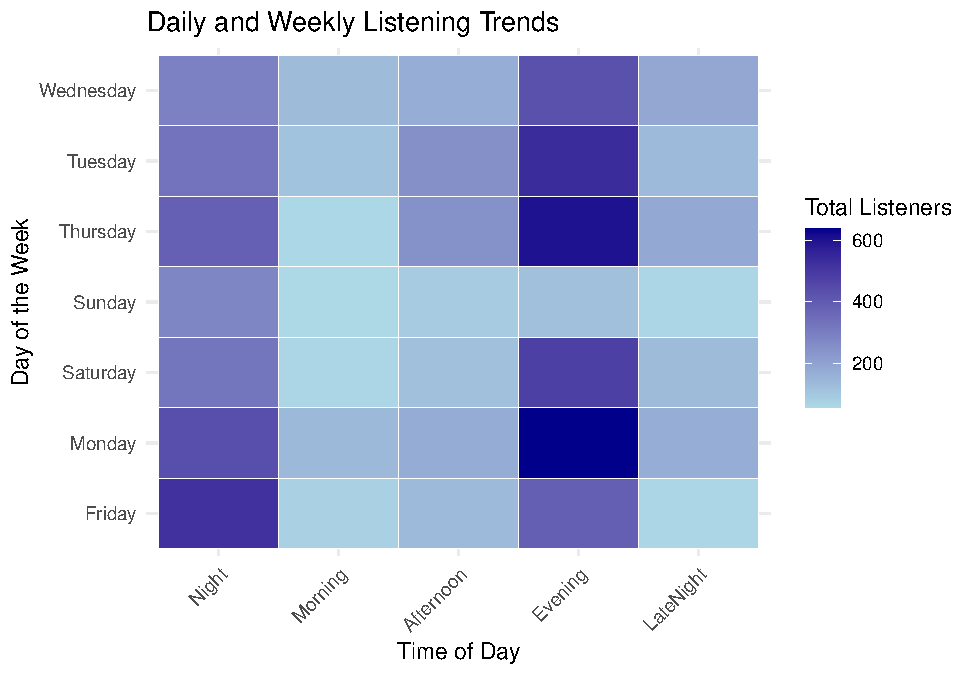
\includegraphics{SpotifyProjectPDF_files/figure-latex/unnamed-chunk-6-1.pdf}

\subsubsection{Session Analysis}\label{session-analysis}

This section provides a detailed analysis of user listening sessions,
summarizing key statistics such as the number of tracks listened to,
session start and end times, and session durations. Session analysis is
vital for understanding user engagement patterns, helping identify how
long users are listening to music and how many tracks they typically
listen to in one sitting. This information can inform strategies for
content delivery, user experience enhancements, and marketing efforts.
By analyzing session durations and track counts, insights can be gained
into user preferences, peak usage times, and overall engagement trends.
These insights can guide the development of features aimed at increasing
user retention and satisfaction, such as personalized recommendations
and session-based promotions.

\begin{Shaded}
\begin{Highlighting}[]
\CommentTok{\# Load necessary libraries}
\FunctionTok{library}\NormalTok{(dplyr)}
\FunctionTok{library}\NormalTok{(knitr)}

\CommentTok{\# Session Analysis}
\NormalTok{session\_analysis }\OtherTok{\textless{}{-}}\NormalTok{ combined\_data }\SpecialCharTok{\%\textgreater{}\%}
  \FunctionTok{group\_by}\NormalTok{(session\_id) }\SpecialCharTok{\%\textgreater{}\%}
  \FunctionTok{summarise}\NormalTok{(}
    \AttributeTok{track\_count =} \FunctionTok{n}\NormalTok{(),                               }\CommentTok{\# Number of tracks in each session}
    \AttributeTok{session\_start\_time =} \FunctionTok{min}\NormalTok{(endTime),               }\CommentTok{\# Start time of session}
    \AttributeTok{session\_end\_time =} \FunctionTok{max}\NormalTok{(endTime),                 }\CommentTok{\# End time of session}
    \AttributeTok{session\_duration =} \FunctionTok{as.numeric}\NormalTok{(}\FunctionTok{difftime}\NormalTok{(session\_end\_time, session\_start\_time, }\AttributeTok{units =} \StringTok{"mins"}\NormalTok{))  }\CommentTok{\# Duration in minutes}
\NormalTok{  ) }

\CommentTok{\# Summarise overall session statistics}
\NormalTok{session\_summary }\OtherTok{\textless{}{-}}\NormalTok{ session\_analysis }\SpecialCharTok{\%\textgreater{}\%}
  \FunctionTok{summarise}\NormalTok{(}
    \AttributeTok{average\_tracks\_per\_session =} \FunctionTok{mean}\NormalTok{(track\_count),}
    \AttributeTok{average\_session\_duration =} \FunctionTok{mean}\NormalTok{(session\_duration),}
    \AttributeTok{total\_sessions =} \FunctionTok{n}\NormalTok{(),}
    \AttributeTok{max\_session\_duration =} \FunctionTok{max}\NormalTok{(session\_duration),}
    \AttributeTok{min\_session\_duration =} \FunctionTok{min}\NormalTok{(session\_duration)}
\NormalTok{  )}

\CommentTok{\# Display summary statistics with kable for better formatting}
\FunctionTok{kable}\NormalTok{(session\_summary, }\AttributeTok{caption =} \StringTok{"Overall Session Analysis"}\NormalTok{, }\AttributeTok{format =} \StringTok{"markdown"}\NormalTok{)}
\end{Highlighting}
\end{Shaded}

\begin{longtable}[]{@{}
  >{\raggedleft\arraybackslash}p{(\columnwidth - 8\tabcolsep) * \real{0.2477}}
  >{\raggedleft\arraybackslash}p{(\columnwidth - 8\tabcolsep) * \real{0.2294}}
  >{\raggedleft\arraybackslash}p{(\columnwidth - 8\tabcolsep) * \real{0.1376}}
  >{\raggedleft\arraybackslash}p{(\columnwidth - 8\tabcolsep) * \real{0.1927}}
  >{\raggedleft\arraybackslash}p{(\columnwidth - 8\tabcolsep) * \real{0.1927}}@{}}
\caption{Overall Session Analysis}\tabularnewline
\toprule\noalign{}
\begin{minipage}[b]{\linewidth}\raggedleft
average\_tracks\_per\_session
\end{minipage} & \begin{minipage}[b]{\linewidth}\raggedleft
average\_session\_duration
\end{minipage} & \begin{minipage}[b]{\linewidth}\raggedleft
total\_sessions
\end{minipage} & \begin{minipage}[b]{\linewidth}\raggedleft
max\_session\_duration
\end{minipage} & \begin{minipage}[b]{\linewidth}\raggedleft
min\_session\_duration
\end{minipage} \\
\midrule\noalign{}
\endfirsthead
\toprule\noalign{}
\begin{minipage}[b]{\linewidth}\raggedleft
average\_tracks\_per\_session
\end{minipage} & \begin{minipage}[b]{\linewidth}\raggedleft
average\_session\_duration
\end{minipage} & \begin{minipage}[b]{\linewidth}\raggedleft
total\_sessions
\end{minipage} & \begin{minipage}[b]{\linewidth}\raggedleft
max\_session\_duration
\end{minipage} & \begin{minipage}[b]{\linewidth}\raggedleft
min\_session\_duration
\end{minipage} \\
\midrule\noalign{}
\endhead
\bottomrule\noalign{}
\endlastfoot
7.998099 & 25.31559 & 1052 & 258 & 0 \\
\end{longtable}

\subsubsection{Frequency of Listening
Analysis}\label{frequency-of-listening-analysis}

This analysis summarizes the most frequently listened-to tracks and also
highlights the top 5 artists based on the total number of listens.
Including the analysis of the top 5 most listened-to artists alongside
track frequency analysis provides a broader understanding of user
preferences and trends in music consumption. This information is
valuable for identifying popular artists and tailoring recommendations,
marketing strategies, and playlists to enhance user engagement. It can
also inform partnerships and promotional opportunities with artists,
driving user satisfaction and retention.

\begin{Shaded}
\begin{Highlighting}[]
\CommentTok{\# Load necessary libraries}
\FunctionTok{library}\NormalTok{(dplyr)      }\CommentTok{\# For data manipulation}
\FunctionTok{library}\NormalTok{(knitr)      }\CommentTok{\# For rendering tables}

\CommentTok{\# Frequency of Listening Analysis}
\NormalTok{track\_frequency }\OtherTok{\textless{}{-}}\NormalTok{ combined\_data }\SpecialCharTok{\%\textgreater{}\%}
  \FunctionTok{group\_by}\NormalTok{(trackName, artistName) }\SpecialCharTok{\%\textgreater{}\%}  \CommentTok{\# Group by track name and artist}
  \FunctionTok{summarise}\NormalTok{(}\AttributeTok{listen\_count =} \FunctionTok{n}\NormalTok{(), }\AttributeTok{.groups =} \StringTok{\textquotesingle{}drop\textquotesingle{}}\NormalTok{) }\SpecialCharTok{\%\textgreater{}\%}  \CommentTok{\# Count listens and drop grouping}
  \FunctionTok{arrange}\NormalTok{(}\FunctionTok{desc}\NormalTok{(listen\_count)) }\SpecialCharTok{\%\textgreater{}\%}  \CommentTok{\# Sort by listen count in descending order}
  \FunctionTok{top\_n}\NormalTok{(}\DecValTok{10}\NormalTok{, listen\_count)  }\CommentTok{\# Show only the top 10 tracks by listen count}

\CommentTok{\# Display frequency of listening with kable for better formatting}
\FunctionTok{kable}\NormalTok{(track\_frequency, }\AttributeTok{caption =} \StringTok{"Top Tracks by Frequency of Listening"}\NormalTok{, }\AttributeTok{format =} \StringTok{"markdown"}\NormalTok{, }
      \AttributeTok{col.names =} \FunctionTok{c}\NormalTok{(}\StringTok{"Track Name"}\NormalTok{, }\StringTok{"Artist Name"}\NormalTok{, }\StringTok{"Listen Count"}\NormalTok{))  }\CommentTok{\# Custom column names}
\end{Highlighting}
\end{Shaded}

\begin{longtable}[]{@{}
  >{\raggedright\arraybackslash}p{(\columnwidth - 4\tabcolsep) * \real{0.6118}}
  >{\raggedright\arraybackslash}p{(\columnwidth - 4\tabcolsep) * \real{0.2353}}
  >{\raggedleft\arraybackslash}p{(\columnwidth - 4\tabcolsep) * \real{0.1529}}@{}}
\caption{Top Tracks by Frequency of Listening}\tabularnewline
\toprule\noalign{}
\begin{minipage}[b]{\linewidth}\raggedright
Track Name
\end{minipage} & \begin{minipage}[b]{\linewidth}\raggedright
Artist Name
\end{minipage} & \begin{minipage}[b]{\linewidth}\raggedleft
Listen Count
\end{minipage} \\
\midrule\noalign{}
\endfirsthead
\toprule\noalign{}
\begin{minipage}[b]{\linewidth}\raggedright
Track Name
\end{minipage} & \begin{minipage}[b]{\linewidth}\raggedright
Artist Name
\end{minipage} & \begin{minipage}[b]{\linewidth}\raggedleft
Listen Count
\end{minipage} \\
\midrule\noalign{}
\endhead
\bottomrule\noalign{}
\endlastfoot
Unwritten & Natasha Bedingfield & 157 \\
Diet Mountain Dew & Lana Del Rey & 121 \\
Is It Over Now? (Taylor's Version) (From The Vault) & Taylor Swift &
115 \\
Murder On The Dancefloor & Sophie Ellis-Bextor & 114 \\
Thank You & Dido & 100 \\
Espresso & Sabrina Carpenter & 99 \\
How You Get The Girl (Taylor's Version) & Taylor Swift & 98 \\
Guilty as Sin? & Taylor Swift & 92 \\
All Too Well (Taylor's Version) & Taylor Swift & 87 \\
Say Don't Go (Taylor's Version) (From The Vault) & Taylor Swift & 82 \\
\end{longtable}

\begin{Shaded}
\begin{Highlighting}[]
\CommentTok{\# Top 5 Most Listened{-}To Artists}
\NormalTok{artist\_frequency }\OtherTok{\textless{}{-}}\NormalTok{ combined\_data }\SpecialCharTok{\%\textgreater{}\%}
  \FunctionTok{group\_by}\NormalTok{(artistName) }\SpecialCharTok{\%\textgreater{}\%}  \CommentTok{\# Group by artist}
  \FunctionTok{summarise}\NormalTok{(}\AttributeTok{artist\_listen\_count =} \FunctionTok{n}\NormalTok{(), }\AttributeTok{.groups =} \StringTok{\textquotesingle{}drop\textquotesingle{}}\NormalTok{) }\SpecialCharTok{\%\textgreater{}\%}  \CommentTok{\# Count listens per artist}
  \FunctionTok{arrange}\NormalTok{(}\FunctionTok{desc}\NormalTok{(artist\_listen\_count)) }\SpecialCharTok{\%\textgreater{}\%}  \CommentTok{\# Sort by listen count in descending order}
  \FunctionTok{top\_n}\NormalTok{(}\DecValTok{5}\NormalTok{, artist\_listen\_count)  }\CommentTok{\# Show only the top 5 artists by listen count}

\CommentTok{\# Display top 5 artists with kable for better formatting}
\FunctionTok{kable}\NormalTok{(artist\_frequency, }\AttributeTok{caption =} \StringTok{"Top 5 Most Listened{-}To Artists"}\NormalTok{, }\AttributeTok{format =} \StringTok{"markdown"}\NormalTok{, }
      \AttributeTok{col.names =} \FunctionTok{c}\NormalTok{(}\StringTok{"Artist Name"}\NormalTok{, }\StringTok{"Listen Count"}\NormalTok{))  }\CommentTok{\# Custom column names}
\end{Highlighting}
\end{Shaded}

\begin{longtable}[]{@{}lr@{}}
\caption{Top 5 Most Listened-To Artists}\tabularnewline
\toprule\noalign{}
Artist Name & Listen Count \\
\midrule\noalign{}
\endfirsthead
\toprule\noalign{}
Artist Name & Listen Count \\
\midrule\noalign{}
\endhead
\bottomrule\noalign{}
\endlastfoot
Taylor Swift & 4115 \\
Lana Del Rey & 226 \\
Sabrina Carpenter & 208 \\
One Direction & 180 \\
Natasha Bedingfield & 177 \\
\end{longtable}

\subsubsection{Investigation of Audio
Features}\label{investigation-of-audio-features}

In this section, we explore the relationships between various audio
features and their impact on user engagement through a correlation
analysis and a statistical test (ANOVA).

\paragraph{Correlation Matrix of Audio
Features}\label{correlation-matrix-of-audio-features}

The \textbf{correlation matrix} provides insights into how different
audio features relate to one another. The features analyzed include:

\begin{itemize}
\tightlist
\item
  \textbf{danceability}: A measure of how suitable a track is for
  dancing, ranging from 0 to 1.
\item
  \textbf{energy}: Represents the intensity and activity of a track,
  also scaled between 0 and 1.
\item
  \textbf{valence}: Indicates the musical positiveness of a track, where
  higher values signify more positive feelings.
\item
  \textbf{msPlayed}: The total milliseconds a track was played,
  representing user engagement.
\end{itemize}

The values in the correlation matrix show the degree of linear
relationship between pairs of features:

\begin{itemize}
\tightlist
\item
  \textbf{Interpretation}:

  \begin{itemize}
  \tightlist
  \item
    A value close to \textbf{1} indicates a strong positive correlation,
    meaning that as one feature increases, the other tends to increase
    as well.
  \item
    A value close to \textbf{-1} indicates a strong negative
    correlation, where an increase in one feature corresponds to a
    decrease in the other.
  \item
    Values around \textbf{0} indicate little to no correlation.
  \end{itemize}
\end{itemize}

\paragraph{ANOVA Results for Energy Levels by Day of the
Week}\label{anova-results-for-energy-levels-by-day-of-the-week}

The \textbf{ANOVA (Analysis of Variance)} results help us understand
whether there are statistically significant differences in energy levels
across different days of the week. The output table includes the
following columns:

\begin{longtable}[]{@{}
  >{\raggedright\arraybackslash}p{(\columnwidth - 2\tabcolsep) * \real{0.5000}}
  >{\raggedright\arraybackslash}p{(\columnwidth - 2\tabcolsep) * \real{0.5000}}@{}}
\toprule\noalign{}
\begin{minipage}[b]{\linewidth}\raggedright
Column
\end{minipage} & \begin{minipage}[b]{\linewidth}\raggedright
Description
\end{minipage} \\
\midrule\noalign{}
\endhead
\bottomrule\noalign{}
\endlastfoot
\textbf{Df} & Degrees of freedom, representing the number of levels in
the factor (day\_of\_week) minus one for the between-group variability
and the residuals. \\
\textbf{Sum Sq} & The total sum of squares for each factor, indicating
the variability attributed to that factor. \\
\textbf{Mean Sq} & Mean square values, calculated as the sum of squares
divided by the respective degrees of freedom. It gives an estimate of
variance associated with each factor. \\
\textbf{F value} & The F-statistic, which is the ratio of the variance
between groups to the variance within groups. A higher F value suggests
a greater degree of variability between the group means relative to the
variability within groups. \\
\textbf{Pr(\textgreater F)} & The p-value associated with the
F-statistic. A lower p-value (typically \textless{} 0.05) indicates a
statistically significant difference between the means of the groups
being compared. \\
\end{longtable}

\begin{itemize}
\tightlist
\item
  \textbf{Interpretation}:

  \begin{itemize}
  \tightlist
  \item
    The ANOVA results indicate that there are significant differences in
    energy levels across different days of the week (p-value = 0.0058),
    suggesting that the day of the week may influence the energy level
    of the music listened to.
  \end{itemize}
\end{itemize}

\paragraph{General Description of the
Code}\label{general-description-of-the-code}

The provided R code performs an investigation into audio features within
the dataset. It consists of the following steps:

\begin{enumerate}
\def\labelenumi{\arabic{enumi}.}
\tightlist
\item
  \textbf{Correlation Analysis}:

  \begin{itemize}
  \tightlist
  \item
    A correlation matrix is calculated for the selected audio features:
    \texttt{danceability}, \texttt{energy}, \texttt{valence}, and
    \texttt{msPlayed}.
  \item
    The correlation matrix is displayed in a neatly formatted table for
    easier interpretation.
  \end{itemize}
\item
  \textbf{Statistical Testing (ANOVA)}:

  \begin{itemize}
  \tightlist
  \item
    An ANOVA test is conducted to determine if there are significant
    differences in energy levels based on the day of the week.
  \item
    The results are summarized in a table that details the degrees of
    freedom, sum of squares, mean squares, F-statistic, and p-value.
  \end{itemize}
\end{enumerate}

Overall, this analysis helps in understanding the interplay between
different audio features and user engagement, providing insights that
can inform further music recommendations or analyses.

\begin{Shaded}
\begin{Highlighting}[]
\CommentTok{\# Load necessary libraries}
\FunctionTok{suppressMessages}\NormalTok{(}\FunctionTok{library}\NormalTok{(dplyr))}
\FunctionTok{suppressMessages}\NormalTok{(}\FunctionTok{library}\NormalTok{(knitr))}
\FunctionTok{suppressMessages}\NormalTok{(}\FunctionTok{library}\NormalTok{(kableExtra))}

\CommentTok{\# 4. Investigation of Audio Features}

\DocumentationTok{\#\# 4.1 Correlation Analysis}
\CommentTok{\# Calculate the correlation matrix for selected features}
\NormalTok{correlation\_matrix }\OtherTok{\textless{}{-}} \FunctionTok{cor}\NormalTok{(combined\_data[, }\FunctionTok{c}\NormalTok{(}\StringTok{"danceability"}\NormalTok{, }\StringTok{"energy"}\NormalTok{, }\StringTok{"valence"}\NormalTok{, }\StringTok{"msPlayed"}\NormalTok{)], }\AttributeTok{use =} \StringTok{"complete.obs"}\NormalTok{)}

\CommentTok{\# Create a kable for the correlation matrix}
\DocumentationTok{\#\#\# Correlation Matrix:}
\FunctionTok{kable}\NormalTok{(correlation\_matrix, }\AttributeTok{digits =} \DecValTok{2}\NormalTok{, }\AttributeTok{caption =} \StringTok{"Correlation Matrix of Audio Features"}\NormalTok{)}
\end{Highlighting}
\end{Shaded}

\begin{longtable}[]{@{}lrrrr@{}}
\caption{Correlation Matrix of Audio Features}\tabularnewline
\toprule\noalign{}
& danceability & energy & valence & msPlayed \\
\midrule\noalign{}
\endfirsthead
\toprule\noalign{}
& danceability & energy & valence & msPlayed \\
\midrule\noalign{}
\endhead
\bottomrule\noalign{}
\endlastfoot
danceability & 1.00 & 0.10 & 0.42 & -0.09 \\
energy & 0.10 & 1.00 & 0.48 & -0.07 \\
valence & 0.42 & 0.48 & 1.00 & -0.13 \\
msPlayed & -0.09 & -0.07 & -0.13 & 1.00 \\
\end{longtable}

\begin{Shaded}
\begin{Highlighting}[]
\DocumentationTok{\#\# 4.2 Statistical Tests}
\CommentTok{\# Perform ANOVA to see if energy levels differ by day of the week}
\NormalTok{anova\_results }\OtherTok{\textless{}{-}} \FunctionTok{aov}\NormalTok{(energy }\SpecialCharTok{\textasciitilde{}}\NormalTok{ day\_of\_week, }\AttributeTok{data =}\NormalTok{ combined\_data)}

\CommentTok{\# Extract ANOVA summary table and convert to a data frame for kable}
\NormalTok{anova\_summary }\OtherTok{\textless{}{-}} \FunctionTok{as.data.frame}\NormalTok{(}\FunctionTok{summary}\NormalTok{(anova\_results)[[}\DecValTok{1}\NormalTok{]])}

\DocumentationTok{\#\#\# ANOVA Results:}
\CommentTok{\# Create a kable for the ANOVA results}
\FunctionTok{kable}\NormalTok{(anova\_summary, }\AttributeTok{caption =} \StringTok{"ANOVA Results for Energy Levels by Day of the Week"}\NormalTok{)}
\end{Highlighting}
\end{Shaded}

\begin{longtable}[]{@{}lrrrrr@{}}
\caption{ANOVA Results for Energy Levels by Day of the
Week}\tabularnewline
\toprule\noalign{}
& Df & Sum Sq & Mean Sq & F value & Pr(\textgreater F) \\
\midrule\noalign{}
\endfirsthead
\toprule\noalign{}
& Df & Sum Sq & Mean Sq & F value & Pr(\textgreater F) \\
\midrule\noalign{}
\endhead
\bottomrule\noalign{}
\endlastfoot
day\_of\_week & 6 & 0.4823289 & 0.0803881 & 3.031174 & 0.0058171 \\
Residuals & 8407 & 222.9575702 & 0.0265205 & NA & NA \\
\end{longtable}

\subsubsection{Mood Labeling and Audio
Features}\label{mood-labeling-and-audio-features}

This analysis focuses on the relationship between audio features and
mood categorization of songs in the Spotify dataset. By examining
features such as valence, energy, and danceability, we aim to classify
each song into specific mood categories. This helps in understanding how
musical elements influence listeners' emotions and preferences.

\begin{enumerate}
\def\labelenumi{\arabic{enumi}.}
\tightlist
\item
  Mood Labeling
\end{enumerate}

We begin by initializing mood labels for each song in the dataset with a
default value of ``Unknown Mood.'' The following criteria are then
applied based on three key audio features:

\begin{itemize}
\tightlist
\item
  \textbf{Valence}: Indicates the musical positiveness conveyed by a
  track. High valence corresponds to a happy or positive mood, while low
  valence suggests a more negative or sad feeling.
\item
  \textbf{Energy}: Reflects the intensity and activity level of a song.
  High energy is associated with fast, loud, and rhythmic tracks, while
  low energy is linked to calm or quiet music.
\item
  \textbf{Danceability}: Represents how suitable a track is for dancing,
  influenced by tempo, rhythm stability, and overall musicality.
\end{itemize}

\begin{enumerate}
\def\labelenumi{\arabic{enumi}.}
\setcounter{enumi}{1}
\tightlist
\item
  Mood Grouping
\end{enumerate}

Once mood labels are assigned, we aggregate the data by mood category to
calculate the average values of danceability, energy, and valence for
each mood group. This provides insights into the characteristics of
songs associated with different moods.

\begin{enumerate}
\def\labelenumi{\arabic{enumi}.}
\setcounter{enumi}{2}
\tightlist
\item
  Heatmap Visualization
\end{enumerate}

To further explore the relationships between audio features, a heatmap
is generated to visualize the correlations among the various audio
features (danceability, energy, valence, loudness, instrumentalness).
This helps to identify patterns and trends in the dataset.

\paragraph{Mood Categories and
Descriptions}\label{mood-categories-and-descriptions}

The following table summarizes the mood categories along with their
descriptions and average audio feature values:

\begin{longtable}[]{@{}
  >{\raggedright\arraybackslash}p{(\columnwidth - 8\tabcolsep) * \real{0.2636}}
  >{\raggedright\arraybackslash}p{(\columnwidth - 8\tabcolsep) * \real{0.2946}}
  >{\raggedright\arraybackslash}p{(\columnwidth - 8\tabcolsep) * \real{0.1395}}
  >{\raggedright\arraybackslash}p{(\columnwidth - 8\tabcolsep) * \real{0.1318}}
  >{\raggedright\arraybackslash}p{(\columnwidth - 8\tabcolsep) * \real{0.1705}}@{}}
\toprule\noalign{}
\begin{minipage}[b]{\linewidth}\raggedright
Mood
\end{minipage} & \begin{minipage}[b]{\linewidth}\raggedright
Description
\end{minipage} & \begin{minipage}[b]{\linewidth}\raggedright
Average Valence
\end{minipage} & \begin{minipage}[b]{\linewidth}\raggedright
Average Energy
\end{minipage} & \begin{minipage}[b]{\linewidth}\raggedright
Average Danceability
\end{minipage} \\
\midrule\noalign{}
\endhead
\bottomrule\noalign{}
\endlastfoot
Happy, Energetic, Uplifting & Joyful and lively songs & \textgreater{}
0.5 & \textgreater{} 0.7 & \textgreater{} 0.5 \\
Sad, Calm, Relaxing & Melancholic and soothing tracks & \textless{} 0.3
& \textless{} 0.3 & \textless{} 0.3 \\
Content, Peaceful, Reflective & Reflective and serene songs &
\textgreater{} 0.5 & \textless{} 0.5 & 0.3 - 0.7 \\
Anxious, Intense, Agitated & High-energy but tense songs & \textless{}
0.3 & \textgreater{} 0.7 & 0.3 - 0.7 \\
Confident, Empowered, Motivational & Uplifting and empowering tracks &
\textgreater{} 0.5 & \textgreater{} 0.7 & \textgreater{} 0.5 \\
Romantic, Warm, Nostalgic & Sentimental and warm songs & \textgreater{}
0.5 & \textless{} 0.5 & \textgreater{} 0.7 \\
Fun, Playful, Lively & Upbeat and entertaining tracks & \textgreater{}
0.4 & \textgreater{} 0.4 & \textgreater{} 0.4 \\
Somber, Reflective, Wistful & Thought-provoking and reflective songs &
\textless{} 0.3 & \textless{} 0.5 & \textgreater{} 0.5 \\
Mellow, Serene, Dreamy & Calm and gentle tracks & \textless{} 0.4 &
\textless{} 0.4 & \textless{} 0.4 \\
Relaxed, Positive, Easy-going & Laid-back and feel-good songs &
\textgreater{} 0.4 & \textless{} 0.4 & \textless{} 0.5 \\
Gritty, Raw, Intense & Raw and intense tracks & \textless{} 0.3 &
\textgreater{} 0.7 & \textless{} 0.3 \\
\end{longtable}

Sources -

\begin{enumerate}
\def\labelenumi{\arabic{enumi}.}
\tightlist
\item
  \url{https://nycdatascience.com/blog/student-works/spotify-metrics-do-you-know-them/}
  2,
  \url{https://towardsdatascience.com/what-makes-a-song-likeable-dbfdb7abe404}
\end{enumerate}

The analysis demonstrates a clear relationship between audio features
and mood categorization in the Spotify dataset. By understanding these
relationships, we can develop better recommendation systems that align
with users' emotional states and enhance their listening experiences.

\begin{Shaded}
\begin{Highlighting}[]
\CommentTok{\# Load necessary libraries}
\FunctionTok{library}\NormalTok{(dplyr)}
\FunctionTok{library}\NormalTok{(kableExtra)}
\FunctionTok{library}\NormalTok{(ggplot2)}
\FunctionTok{library}\NormalTok{(reshape2)}

\CommentTok{\# 5.1 Refined Mood Labeling}
\CommentTok{\# Initialize the mood\_labels vector}
\NormalTok{mood\_labels }\OtherTok{\textless{}{-}} \FunctionTok{character}\NormalTok{(}\FunctionTok{nrow}\NormalTok{(combined\_data))}

\CommentTok{\# Assign moods based on the revised conditions informed by music research}
\ControlFlowTok{for}\NormalTok{ (i }\ControlFlowTok{in} \DecValTok{1}\SpecialCharTok{:}\FunctionTok{nrow}\NormalTok{(combined\_data)) \{}
\NormalTok{  row }\OtherTok{\textless{}{-}}\NormalTok{ combined\_data[i, ]}
  
  \CommentTok{\# Assigning moods based on research insights}
  \ControlFlowTok{if}\NormalTok{ (row[}\StringTok{\textquotesingle{}valence\textquotesingle{}}\NormalTok{] }\SpecialCharTok{\textgreater{}} \FloatTok{0.6} \SpecialCharTok{\&\&}\NormalTok{ row[}\StringTok{\textquotesingle{}energy\textquotesingle{}}\NormalTok{] }\SpecialCharTok{\textgreater{}} \FloatTok{0.7} \SpecialCharTok{\&\&}\NormalTok{ row[}\StringTok{\textquotesingle{}danceability\textquotesingle{}}\NormalTok{] }\SpecialCharTok{\textgreater{}} \FloatTok{0.5}\NormalTok{) \{}
\NormalTok{    mood\_labels[i] }\OtherTok{\textless{}{-}} \StringTok{\textquotesingle{}Happy, Energetic, Uplifting\textquotesingle{}}  \CommentTok{\# Bright, fast{-}paced songs}
\NormalTok{  \} }\ControlFlowTok{else} \ControlFlowTok{if}\NormalTok{ (row[}\StringTok{\textquotesingle{}valence\textquotesingle{}}\NormalTok{] }\SpecialCharTok{\textless{}} \FloatTok{0.3} \SpecialCharTok{\&\&}\NormalTok{ row[}\StringTok{\textquotesingle{}energy\textquotesingle{}}\NormalTok{] }\SpecialCharTok{\textless{}} \FloatTok{0.4} \SpecialCharTok{\&\&}\NormalTok{ row[}\StringTok{\textquotesingle{}danceability\textquotesingle{}}\NormalTok{] }\SpecialCharTok{\textless{}} \FloatTok{0.4}\NormalTok{) \{}
\NormalTok{    mood\_labels[i] }\OtherTok{\textless{}{-}} \StringTok{\textquotesingle{}Sad, Calm, Relaxing\textquotesingle{}}  \CommentTok{\# Slow, somber songs}
\NormalTok{  \} }\ControlFlowTok{else} \ControlFlowTok{if}\NormalTok{ (row[}\StringTok{\textquotesingle{}valence\textquotesingle{}}\NormalTok{] }\SpecialCharTok{\textgreater{}=} \FloatTok{0.4} \SpecialCharTok{\&\&}\NormalTok{ row[}\StringTok{\textquotesingle{}valence\textquotesingle{}}\NormalTok{] }\SpecialCharTok{\textless{}} \FloatTok{0.6} \SpecialCharTok{\&\&}\NormalTok{ row[}\StringTok{\textquotesingle{}energy\textquotesingle{}}\NormalTok{] }\SpecialCharTok{\textless{}} \FloatTok{0.6} \SpecialCharTok{\&\&}\NormalTok{ row[}\StringTok{\textquotesingle{}danceability\textquotesingle{}}\NormalTok{] }\SpecialCharTok{\textgreater{}=} \FloatTok{0.4}\NormalTok{) \{}
\NormalTok{    mood\_labels[i] }\OtherTok{\textless{}{-}} \StringTok{\textquotesingle{}Content, Peaceful, Reflective\textquotesingle{}}  \CommentTok{\# Moderate energy, soothing}
\NormalTok{  \} }\ControlFlowTok{else} \ControlFlowTok{if}\NormalTok{ (row[}\StringTok{\textquotesingle{}valence\textquotesingle{}}\NormalTok{] }\SpecialCharTok{\textless{}} \FloatTok{0.3} \SpecialCharTok{\&\&}\NormalTok{ row[}\StringTok{\textquotesingle{}energy\textquotesingle{}}\NormalTok{] }\SpecialCharTok{\textgreater{}=} \FloatTok{0.5} \SpecialCharTok{\&\&}\NormalTok{ row[}\StringTok{\textquotesingle{}danceability\textquotesingle{}}\NormalTok{] }\SpecialCharTok{\textgreater{}=} \FloatTok{0.4}\NormalTok{) \{}
\NormalTok{    mood\_labels[i] }\OtherTok{\textless{}{-}} \StringTok{\textquotesingle{}Anxious, Intense, Agitated\textquotesingle{}}  \CommentTok{\# Intense, faster songs}
\NormalTok{  \} }\ControlFlowTok{else} \ControlFlowTok{if}\NormalTok{ (row[}\StringTok{\textquotesingle{}valence\textquotesingle{}}\NormalTok{] }\SpecialCharTok{\textgreater{}=} \FloatTok{0.5} \SpecialCharTok{\&\&}\NormalTok{ row[}\StringTok{\textquotesingle{}energy\textquotesingle{}}\NormalTok{] }\SpecialCharTok{\textgreater{}=} \FloatTok{0.6} \SpecialCharTok{\&\&}\NormalTok{ row[}\StringTok{\textquotesingle{}danceability\textquotesingle{}}\NormalTok{] }\SpecialCharTok{\textgreater{}=} \FloatTok{0.4}\NormalTok{) \{}
\NormalTok{    mood\_labels[i] }\OtherTok{\textless{}{-}} \StringTok{\textquotesingle{}Confident, Empowered, Motivational\textquotesingle{}}  \CommentTok{\# Uplifting, strong beats}
\NormalTok{  \} }\ControlFlowTok{else} \ControlFlowTok{if}\NormalTok{ (row[}\StringTok{\textquotesingle{}valence\textquotesingle{}}\NormalTok{] }\SpecialCharTok{\textgreater{}=} \FloatTok{0.5} \SpecialCharTok{\&\&}\NormalTok{ row[}\StringTok{\textquotesingle{}energy\textquotesingle{}}\NormalTok{] }\SpecialCharTok{\textless{}} \FloatTok{0.5} \SpecialCharTok{\&\&}\NormalTok{ row[}\StringTok{\textquotesingle{}danceability\textquotesingle{}}\NormalTok{] }\SpecialCharTok{\textgreater{}} \FloatTok{0.5}\NormalTok{) \{}
\NormalTok{    mood\_labels[i] }\OtherTok{\textless{}{-}} \StringTok{\textquotesingle{}Romantic, Warm, Nostalgic\textquotesingle{}}  \CommentTok{\# Slow, sentimental}
\NormalTok{  \} }\ControlFlowTok{else} \ControlFlowTok{if}\NormalTok{ (row[}\StringTok{\textquotesingle{}valence\textquotesingle{}}\NormalTok{] }\SpecialCharTok{\textgreater{}=} \FloatTok{0.4} \SpecialCharTok{\&\&}\NormalTok{ row[}\StringTok{\textquotesingle{}energy\textquotesingle{}}\NormalTok{] }\SpecialCharTok{\textgreater{}=} \FloatTok{0.4} \SpecialCharTok{\&\&}\NormalTok{ row[}\StringTok{\textquotesingle{}danceability\textquotesingle{}}\NormalTok{] }\SpecialCharTok{\textgreater{}} \FloatTok{0.5}\NormalTok{) \{}
\NormalTok{    mood\_labels[i] }\OtherTok{\textless{}{-}} \StringTok{\textquotesingle{}Fun, Playful, Lively\textquotesingle{}}  \CommentTok{\# Upbeat and catchy}
\NormalTok{  \} }\ControlFlowTok{else} \ControlFlowTok{if}\NormalTok{ (row[}\StringTok{\textquotesingle{}valence\textquotesingle{}}\NormalTok{] }\SpecialCharTok{\textless{}} \FloatTok{0.4} \SpecialCharTok{\&\&}\NormalTok{ row[}\StringTok{\textquotesingle{}energy\textquotesingle{}}\NormalTok{] }\SpecialCharTok{\textless{}} \FloatTok{0.5} \SpecialCharTok{\&\&}\NormalTok{ row[}\StringTok{\textquotesingle{}danceability\textquotesingle{}}\NormalTok{] }\SpecialCharTok{\textgreater{}=} \FloatTok{0.4}\NormalTok{) \{}
\NormalTok{    mood\_labels[i] }\OtherTok{\textless{}{-}} \StringTok{\textquotesingle{}Somber, Reflective, Wistful\textquotesingle{}}  \CommentTok{\# Thoughtful and slow}
\NormalTok{  \} }\ControlFlowTok{else} \ControlFlowTok{if}\NormalTok{ (row[}\StringTok{\textquotesingle{}valence\textquotesingle{}}\NormalTok{] }\SpecialCharTok{\textless{}} \FloatTok{0.4} \SpecialCharTok{\&\&}\NormalTok{ row[}\StringTok{\textquotesingle{}energy\textquotesingle{}}\NormalTok{] }\SpecialCharTok{\textless{}} \FloatTok{0.4} \SpecialCharTok{\&\&}\NormalTok{ row[}\StringTok{\textquotesingle{}danceability\textquotesingle{}}\NormalTok{] }\SpecialCharTok{\textless{}} \FloatTok{0.4}\NormalTok{) \{}
\NormalTok{    mood\_labels[i] }\OtherTok{\textless{}{-}} \StringTok{\textquotesingle{}Mellow, Serene, Dreamy\textquotesingle{}}  \CommentTok{\# Chill and laid{-}back}
\NormalTok{  \} }\ControlFlowTok{else} \ControlFlowTok{if}\NormalTok{ (row[}\StringTok{\textquotesingle{}valence\textquotesingle{}}\NormalTok{] }\SpecialCharTok{\textgreater{}=} \FloatTok{0.3} \SpecialCharTok{\&\&}\NormalTok{ row[}\StringTok{\textquotesingle{}energy\textquotesingle{}}\NormalTok{] }\SpecialCharTok{\textless{}} \FloatTok{0.6} \SpecialCharTok{\&\&}\NormalTok{ row[}\StringTok{\textquotesingle{}danceability\textquotesingle{}}\NormalTok{] }\SpecialCharTok{\textless{}} \FloatTok{0.5}\NormalTok{) \{}
\NormalTok{    mood\_labels[i] }\OtherTok{\textless{}{-}} \StringTok{\textquotesingle{}Relaxed, Positive, Easy{-}going\textquotesingle{}}  \CommentTok{\# Calm but cheerful}
\NormalTok{  \} }\ControlFlowTok{else} \ControlFlowTok{if}\NormalTok{ (row[}\StringTok{\textquotesingle{}valence\textquotesingle{}}\NormalTok{] }\SpecialCharTok{\textless{}} \FloatTok{0.3} \SpecialCharTok{\&\&}\NormalTok{ row[}\StringTok{\textquotesingle{}energy\textquotesingle{}}\NormalTok{] }\SpecialCharTok{\textgreater{}=} \FloatTok{0.4} \SpecialCharTok{\&\&}\NormalTok{ row[}\StringTok{\textquotesingle{}danceability\textquotesingle{}}\NormalTok{] }\SpecialCharTok{\textless{}} \FloatTok{0.4}\NormalTok{) \{}
\NormalTok{    mood\_labels[i] }\OtherTok{\textless{}{-}} \StringTok{\textquotesingle{}Gritty, Raw, Intense\textquotesingle{}}  \CommentTok{\# Aggressive or edgy}
\NormalTok{  \} }\ControlFlowTok{else}\NormalTok{ \{}
\NormalTok{    mood\_labels[i] }\OtherTok{\textless{}{-}} \StringTok{\textquotesingle{}Balanced, Neutral, Easy{-}going\textquotesingle{}}  \CommentTok{\# General category to cover remaining cases}
\NormalTok{  \}}
\NormalTok{\}}

\CommentTok{\# Add mood labels to the dataset}
\NormalTok{combined\_data}\SpecialCharTok{$}\NormalTok{mood }\OtherTok{\textless{}{-}}\NormalTok{ mood\_labels}

\CommentTok{\# 5.2 Mood Grouping}
\CommentTok{\# Group songs based on mood and calculate mean values for audio features}
\NormalTok{mood\_grouped }\OtherTok{\textless{}{-}}\NormalTok{ combined\_data }\SpecialCharTok{\%\textgreater{}\%}
  \FunctionTok{group\_by}\NormalTok{(mood) }\SpecialCharTok{\%\textgreater{}\%}
  \FunctionTok{summarise}\NormalTok{(}
    \AttributeTok{avg\_danceability =} \FunctionTok{mean}\NormalTok{(danceability, }\AttributeTok{na.rm =} \ConstantTok{TRUE}\NormalTok{),}
    \AttributeTok{avg\_energy =} \FunctionTok{mean}\NormalTok{(energy, }\AttributeTok{na.rm =} \ConstantTok{TRUE}\NormalTok{),}
    \AttributeTok{avg\_valence =} \FunctionTok{mean}\NormalTok{(valence, }\AttributeTok{na.rm =} \ConstantTok{TRUE}\NormalTok{),}
    \AttributeTok{count =} \FunctionTok{n}\NormalTok{()}
\NormalTok{  )}

\CommentTok{\# Display mood grouping results with kable}
\NormalTok{mood\_grouped }\SpecialCharTok{\%\textgreater{}\%}
  \FunctionTok{kable}\NormalTok{(}\AttributeTok{digits =} \DecValTok{2}\NormalTok{, }\AttributeTok{caption =} \StringTok{"Average Audio Features by Mood Group"}\NormalTok{) }\SpecialCharTok{\%\textgreater{}\%}
  \FunctionTok{kable\_styling}\NormalTok{(}\AttributeTok{full\_width =}\NormalTok{ F, }\AttributeTok{position =} \StringTok{"left"}\NormalTok{, }\AttributeTok{bootstrap\_options =} \FunctionTok{c}\NormalTok{(}\StringTok{"striped"}\NormalTok{, }\StringTok{"hover"}\NormalTok{, }\StringTok{"condensed"}\NormalTok{))}
\end{Highlighting}
\end{Shaded}

\begin{longtable}[l]{lrrrr}
\caption{\label{tab:unnamed-chunk-10}Average Audio Features by Mood Group}\\
\toprule
mood & avg\_danceability & avg\_energy & avg\_valence & count\\
\midrule
Anxious, Intense, Agitated & 0.58 & 0.65 & 0.21 & 1209\\
Balanced, Neutral, Easy-going & 0.56 & 0.68 & 0.39 & 746\\
Confident, Empowered, Motivational & 0.66 & 0.73 & 0.61 & 2068\\
Content, Peaceful, Reflective & 0.64 & 0.48 & 0.48 & 541\\
Fun, Playful, Lively & 0.66 & 0.67 & 0.57 & 886\\
\addlinespace
Gritty, Raw, Intense & 0.36 & 0.57 & 0.18 & 85\\
Happy, Energetic, Uplifting & 0.69 & 0.82 & 0.76 & 1926\\
Mellow, Serene, Dreamy & 0.38 & 0.28 & 0.33 & 7\\
Relaxed, Positive, Easy-going & 0.37 & 0.47 & 0.50 & 74\\
Romantic, Warm, Nostalgic & 0.65 & 0.43 & 0.78 & 45\\
\addlinespace
Sad, Calm, Relaxing & 0.33 & 0.27 & 0.16 & 35\\
Somber, Reflective, Wistful & 0.60 & 0.39 & 0.21 & 792\\
\bottomrule
\end{longtable}

\begin{Shaded}
\begin{Highlighting}[]
\CommentTok{\# 5.3 Heatmap of Audio Feature Correlation}
\CommentTok{\# Calculate the correlation matrix of audio features}
\NormalTok{audio\_features }\OtherTok{\textless{}{-}}\NormalTok{ combined\_data }\SpecialCharTok{\%\textgreater{}\%} \FunctionTok{select}\NormalTok{(danceability, energy, valence, loudness, instrumentalness)}
\NormalTok{correlation\_matrix }\OtherTok{\textless{}{-}} \FunctionTok{cor}\NormalTok{(audio\_features, }\AttributeTok{use =} \StringTok{"complete.obs"}\NormalTok{)}

\CommentTok{\# Melt the correlation matrix for heatmap}
\NormalTok{correlation\_melted }\OtherTok{\textless{}{-}} \FunctionTok{melt}\NormalTok{(correlation\_matrix)}

\CommentTok{\# Create the heatmap}
\FunctionTok{ggplot}\NormalTok{(correlation\_melted, }\FunctionTok{aes}\NormalTok{(Var1, Var2, }\AttributeTok{fill =}\NormalTok{ value)) }\SpecialCharTok{+}
  \FunctionTok{geom\_tile}\NormalTok{(}\AttributeTok{color =} \StringTok{"white"}\NormalTok{) }\SpecialCharTok{+}
  \FunctionTok{scale\_fill\_gradient2}\NormalTok{(}\AttributeTok{low =} \StringTok{"blue"}\NormalTok{, }\AttributeTok{mid =} \StringTok{"white"}\NormalTok{, }\AttributeTok{high =} \StringTok{"red"}\NormalTok{, }\AttributeTok{midpoint =} \DecValTok{0}\NormalTok{, }\AttributeTok{limit =} \FunctionTok{c}\NormalTok{(}\SpecialCharTok{{-}}\DecValTok{1}\NormalTok{, }\DecValTok{1}\NormalTok{), }\AttributeTok{name =} \StringTok{"Correlation"}\NormalTok{) }\SpecialCharTok{+}
  \FunctionTok{theme\_minimal}\NormalTok{() }\SpecialCharTok{+}
  \FunctionTok{labs}\NormalTok{(}\AttributeTok{title =} \StringTok{"Heatmap of Audio Feature Correlation"}\NormalTok{, }\AttributeTok{x =} \StringTok{"Features"}\NormalTok{, }\AttributeTok{y =} \StringTok{"Features"}\NormalTok{) }\SpecialCharTok{+}
  \FunctionTok{theme}\NormalTok{(}\AttributeTok{axis.text.x =} \FunctionTok{element\_text}\NormalTok{(}\AttributeTok{angle =} \DecValTok{45}\NormalTok{, }\AttributeTok{vjust =} \FloatTok{0.5}\NormalTok{, }\AttributeTok{hjust =} \DecValTok{1}\NormalTok{))}
\end{Highlighting}
\end{Shaded}

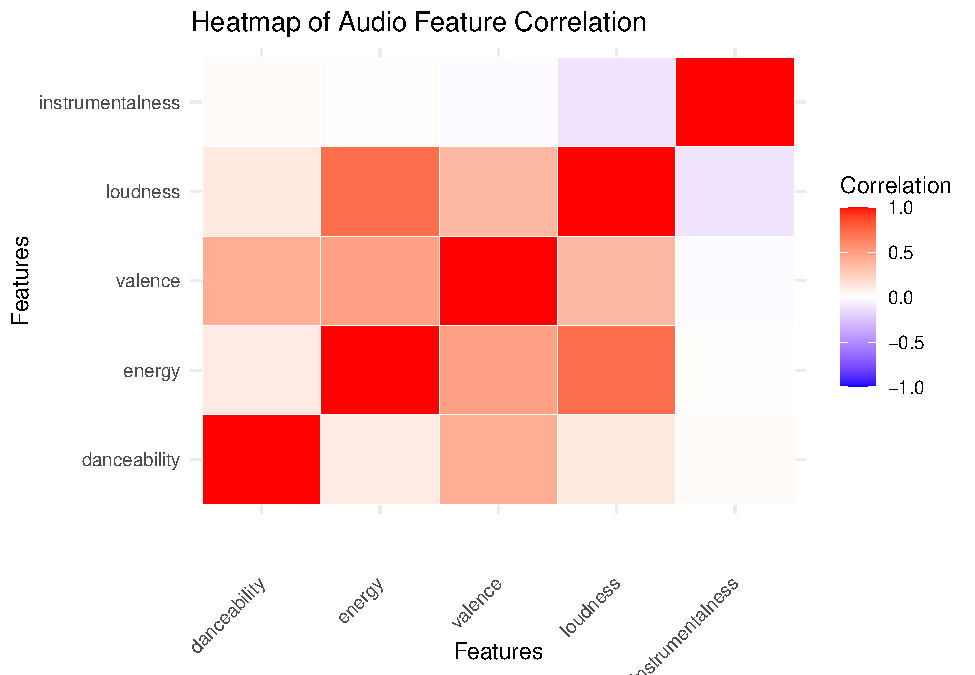
\includegraphics{SpotifyProjectPDF_files/figure-latex/unnamed-chunk-10-1.pdf}

\begin{Shaded}
\begin{Highlighting}[]
\CommentTok{\# 5.4 Display the First Few Rows of the Data}
\NormalTok{combined\_data }\SpecialCharTok{\%\textgreater{}\%}
  \FunctionTok{head}\NormalTok{(}\DecValTok{5}\NormalTok{) }\SpecialCharTok{\%\textgreater{}\%}
  \FunctionTok{kable}\NormalTok{(}\AttributeTok{caption =} \StringTok{"First Five Rows of Combined Data"}\NormalTok{, }\AttributeTok{digits =} \DecValTok{2}\NormalTok{) }\SpecialCharTok{\%\textgreater{}\%}
  \FunctionTok{kable\_styling}\NormalTok{(}\AttributeTok{full\_width =}\NormalTok{ F, }\AttributeTok{position =} \StringTok{"left"}\NormalTok{, }\AttributeTok{bootstrap\_options =} \FunctionTok{c}\NormalTok{(}\StringTok{"striped"}\NormalTok{, }\StringTok{"hover"}\NormalTok{, }\StringTok{"condensed"}\NormalTok{))}
\end{Highlighting}
\end{Shaded}

\begin{longtable}[l]{lllrrrrrrllrll}
\caption{\label{tab:unnamed-chunk-10}First Five Rows of Combined Data}\\
\toprule
endTime & artistName & trackName & msPlayed & danceability & energy & valence & loudness & instrumentalness & day\_of\_week & time\_of\_day & session\_id & listener\_category & mood\\
\midrule
2023-10-11 23:26:00 & Taylor Swift & New Romantics & 198489 & 0.65 & 0.85 & 0.72 & -5.94 & 0 & Wednesday & LateNight & 1 & Super Listeners & Happy, Energetic, Uplifting\\
2023-10-12 00:49:00 & Taylor Swift & New Romantics & 31864 & 0.65 & 0.85 & 0.72 & -5.94 & 0 & Thursday & Night & 2 & Super Listeners & Happy, Energetic, Uplifting\\
2023-10-12 00:54:00 & Taylor Swift & The Story Of Us (Taylor's Version) & 267653 & 0.52 & 0.78 & 0.55 & -2.64 & 0 & Thursday & Night & 2 & Super Listeners & Confident, Empowered, Motivational\\
2023-10-12 00:58:00 & Taylor Swift & End Game & 244826 & 0.65 & 0.59 & 0.15 & -6.24 & 0 & Thursday & Night & 2 & Super Listeners & Anxious, Intense, Agitated\\
2023-10-12 00:59:00 & Taylor Swift & All You Had To Do Was Stay & 34933 & 0.59 & 0.71 & 0.54 & -5.61 & 0 & Thursday & Night & 2 & Super Listeners & Confident, Empowered, Motivational\\
\bottomrule
\end{longtable}

\begin{Shaded}
\begin{Highlighting}[]
\NormalTok{output\_path }\OtherTok{\textless{}{-}} \StringTok{"combined\_data.csv"}
\FunctionTok{write.csv}\NormalTok{(combined\_data, }\AttributeTok{file =}\NormalTok{ output\_path, }\AttributeTok{row.names =} \ConstantTok{FALSE}\NormalTok{)}
\end{Highlighting}
\end{Shaded}

\subsection{Part 4: Data Visualization}\label{part-4-data-visualization}

\subsubsection{Mood Distribution in Spotify Listening
History}\label{mood-distribution-in-spotify-listening-history}

The pie chart represents the distribution of different mood categories
in the Spotify listening history. Each slice corresponds to a specific
mood label, showing how frequently tracks associated with that mood were
played. The chart provides a clear visual of the relative proportions of
each mood, offering an overview of the listener's preferences across
various emotional tones.

The insights drawn from this chart can help identify which mood
categories dominate the listening habits. A larger slice for a
particular mood indicates a strong preference for that emotional tone,
such as Happy, energetic, or uplifting music. Conversely, a more
balanced distribution suggests a diverse taste across multiple moods.
Understanding this distribution is useful for building mood-based music
recommendations or exploring how the listener's preferences shift over
different periods.

\begin{Shaded}
\begin{Highlighting}[]
\CommentTok{\# Create a summarized data frame for mood counts}
\NormalTok{mood\_distribution }\OtherTok{\textless{}{-}}\NormalTok{ combined\_data }\SpecialCharTok{\%\textgreater{}\%}
  \FunctionTok{group\_by}\NormalTok{(mood) }\SpecialCharTok{\%\textgreater{}\%}
  \FunctionTok{summarise}\NormalTok{(}\AttributeTok{count =} \FunctionTok{n}\NormalTok{())}

\CommentTok{\# Generate a pie chart}
\FunctionTok{ggplot}\NormalTok{(mood\_distribution, }\FunctionTok{aes}\NormalTok{(}\AttributeTok{x =} \StringTok{""}\NormalTok{, }\AttributeTok{y =}\NormalTok{ count, }\AttributeTok{fill =}\NormalTok{ mood)) }\SpecialCharTok{+}
  \FunctionTok{geom\_bar}\NormalTok{(}\AttributeTok{stat =} \StringTok{"identity"}\NormalTok{, }\AttributeTok{width =} \DecValTok{1}\NormalTok{) }\SpecialCharTok{+}
  \FunctionTok{coord\_polar}\NormalTok{(}\StringTok{"y"}\NormalTok{) }\SpecialCharTok{+}
  \FunctionTok{labs}\NormalTok{(}
    \AttributeTok{title =} \StringTok{"Mood Distribution in Spotify Listening History"}\NormalTok{,}
    \AttributeTok{x =} \ConstantTok{NULL}\NormalTok{,}
    \AttributeTok{y =} \ConstantTok{NULL}
\NormalTok{  ) }\SpecialCharTok{+}
  \FunctionTok{theme\_minimal}\NormalTok{() }\SpecialCharTok{+}
  \FunctionTok{theme}\NormalTok{(}\AttributeTok{axis.text.x =} \FunctionTok{element\_blank}\NormalTok{(), }\AttributeTok{axis.ticks =} \FunctionTok{element\_blank}\NormalTok{()) }\SpecialCharTok{+}
  \FunctionTok{scale\_fill\_brewer}\NormalTok{(}\AttributeTok{palette =} \StringTok{"Set3"}\NormalTok{)}
\end{Highlighting}
\end{Shaded}

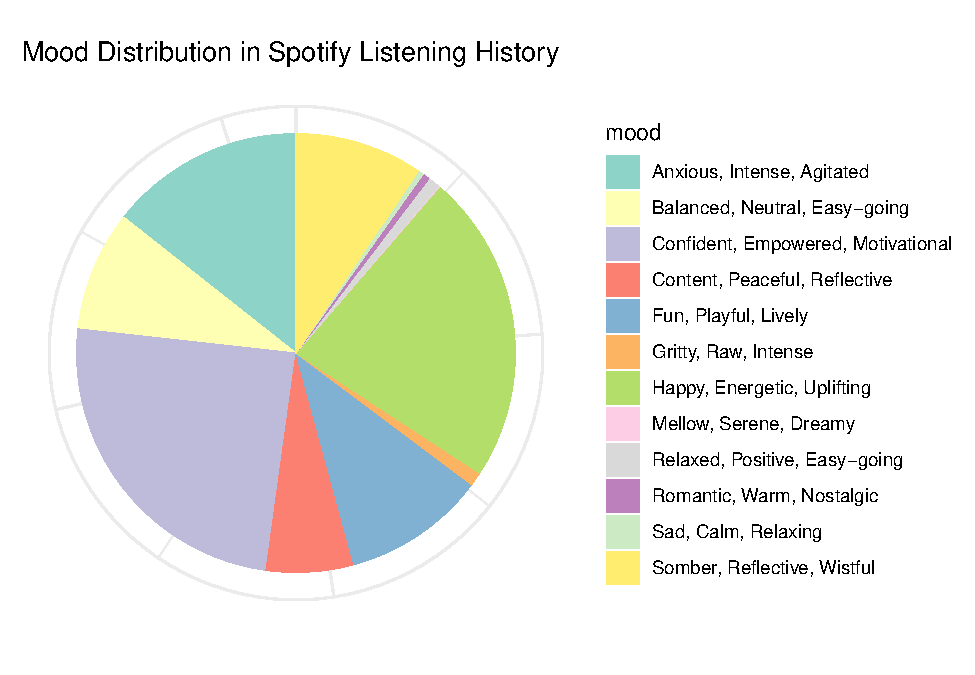
\includegraphics{SpotifyProjectPDF_files/figure-latex/unnamed-chunk-11-1.pdf}

\subsubsection{Total Listening Time Over
Time}\label{total-listening-time-over-time}

The line graph visualizes the total listening time in minutes over a
period, aggregated by day. Each point on the x-axis represents a
specific date, while the y-axis indicates the total listening duration
for that day. A smooth trend line has been added to highlight general
patterns in listening habits, along with a horizontal dashed line to
mark the average daily listening time. The graph's clean design, with a
soft blue line and minimal background, enhances readability and focuses
attention on key trends.

The insights from this graph help identify variations in daily listening
behavior. Peaks in the graph suggest days with significantly higher
engagement, possibly indicating special occasions or mood changes that
led to more music consumption. Conversely, troughs might reflect less
active listening periods. The smooth trend line allows for an easy
observation of overall listening patterns, while the average line offers
a benchmark to quickly assess how daily behavior compares to typical
listening habits. This information can be useful for understanding
shifts in music engagement over time, potentially uncovering seasonal or
weekly trends.

\begin{Shaded}
\begin{Highlighting}[]
\FunctionTok{library}\NormalTok{(ggplot2)}
\FunctionTok{library}\NormalTok{(dplyr)}

\CommentTok{\# Aggregate data by day and convert msPlayed to minutes}
\NormalTok{daily\_listening }\OtherTok{\textless{}{-}}\NormalTok{ combined\_data }\SpecialCharTok{\%\textgreater{}\%}
  \FunctionTok{mutate}\NormalTok{(}\AttributeTok{endTime =} \FunctionTok{as.Date}\NormalTok{(endTime)) }\SpecialCharTok{\%\textgreater{}\%}
  \FunctionTok{group\_by}\NormalTok{(endTime) }\SpecialCharTok{\%\textgreater{}\%}
  \FunctionTok{summarise}\NormalTok{(}\AttributeTok{Total\_msPlayed =} \FunctionTok{sum}\NormalTok{(msPlayed) }\SpecialCharTok{/} \DecValTok{60000}\NormalTok{) }\CommentTok{\# Convert to minutes}

\CommentTok{\# Calculate the average listening time}
\NormalTok{average\_listening }\OtherTok{\textless{}{-}} \FunctionTok{mean}\NormalTok{(daily\_listening}\SpecialCharTok{$}\NormalTok{Total\_msPlayed)}

\CommentTok{\# Determine the y{-}axis limits}
\NormalTok{y\_limit }\OtherTok{\textless{}{-}} \FunctionTok{c}\NormalTok{(}\DecValTok{0}\NormalTok{, }\FunctionTok{max}\NormalTok{(daily\_listening}\SpecialCharTok{$}\NormalTok{Total\_msPlayed) }\SpecialCharTok{*} \FloatTok{1.1}\NormalTok{)  }\CommentTok{\# Set limit with a 10\% increase for better view}

\CommentTok{\# Create a unique and visually appealing line graph without points and adjusted scale}
\FunctionTok{ggplot}\NormalTok{(daily\_listening, }\FunctionTok{aes}\NormalTok{(}\AttributeTok{x =}\NormalTok{ endTime, }\AttributeTok{y =}\NormalTok{ Total\_msPlayed)) }\SpecialCharTok{+}
  \FunctionTok{geom\_line}\NormalTok{(}\AttributeTok{color =} \StringTok{"\#4F81BD"}\NormalTok{, }\AttributeTok{linewidth =} \FloatTok{1.2}\NormalTok{) }\SpecialCharTok{+}  \CommentTok{\# Soft blue line}
  \FunctionTok{geom\_smooth}\NormalTok{(}\AttributeTok{method =} \StringTok{"loess"}\NormalTok{, }\AttributeTok{formula =}\NormalTok{ y }\SpecialCharTok{\textasciitilde{}}\NormalTok{ x, }\AttributeTok{span =} \FloatTok{0.5}\NormalTok{, }\AttributeTok{color =} \StringTok{"\#D95319"}\NormalTok{, }
              \AttributeTok{fill =} \StringTok{"\#F0AD4E"}\NormalTok{, }\AttributeTok{alpha =} \FloatTok{0.3}\NormalTok{, }\AttributeTok{se =} \ConstantTok{TRUE}\NormalTok{) }\SpecialCharTok{+}  \CommentTok{\# Explicit formula}
  \FunctionTok{geom\_hline}\NormalTok{(}\AttributeTok{yintercept =}\NormalTok{ average\_listening, }\AttributeTok{linetype =} \StringTok{"dashed"}\NormalTok{, }\AttributeTok{color =} \StringTok{"black"}\NormalTok{, }\AttributeTok{linewidth =} \FloatTok{1.2}\NormalTok{) }\SpecialCharTok{+}  \CommentTok{\# Average line}
  \FunctionTok{labs}\NormalTok{(}\AttributeTok{title =} \StringTok{"Total Listening Time Over Time (in Minutes)"}\NormalTok{,}
       \AttributeTok{x =} \StringTok{"Date"}\NormalTok{, }\AttributeTok{y =} \StringTok{"Total Listening Time (minutes)"}\NormalTok{) }\SpecialCharTok{+}
  \FunctionTok{annotate}\NormalTok{(}\StringTok{"text"}\NormalTok{, }\AttributeTok{x =} \FunctionTok{max}\NormalTok{(daily\_listening}\SpecialCharTok{$}\NormalTok{endTime), }\AttributeTok{y =}\NormalTok{ average\_listening }\SpecialCharTok{+} \DecValTok{40}\NormalTok{,  }\CommentTok{\# Move annotation higher}
           \AttributeTok{label =} \FunctionTok{paste}\NormalTok{(}\StringTok{"Average:"}\NormalTok{, }\FunctionTok{round}\NormalTok{(average\_listening, }\DecValTok{2}\NormalTok{)), }
           \AttributeTok{color =} \StringTok{"black"}\NormalTok{, }\AttributeTok{hjust =} \DecValTok{1}\NormalTok{, }\AttributeTok{size =} \DecValTok{5}\NormalTok{, }\AttributeTok{alpha =} \FloatTok{0.8}\NormalTok{) }\SpecialCharTok{+}  \CommentTok{\# Average annotation with transparency}
  \FunctionTok{scale\_y\_continuous}\NormalTok{(}\AttributeTok{limits =}\NormalTok{ y\_limit) }\SpecialCharTok{+}  \CommentTok{\# Set y{-}axis limits}
  \FunctionTok{theme\_minimal}\NormalTok{(}\AttributeTok{base\_size =} \DecValTok{15}\NormalTok{) }\SpecialCharTok{+}  \CommentTok{\# Increase base font size for readability}
  \FunctionTok{theme}\NormalTok{(}\AttributeTok{panel.grid.major =} \FunctionTok{element\_line}\NormalTok{(}\AttributeTok{color =} \StringTok{"\#EAEAEA"}\NormalTok{),  }\CommentTok{\# Light grid lines}
        \AttributeTok{panel.grid.minor =} \FunctionTok{element\_blank}\NormalTok{(),  }\CommentTok{\# No minor grid lines}
        \AttributeTok{plot.background =} \FunctionTok{element\_rect}\NormalTok{(}\AttributeTok{fill =} \StringTok{"\#F9F9F9"}\NormalTok{, }\AttributeTok{color =} \ConstantTok{NA}\NormalTok{),  }\CommentTok{\# Soft background}
        \AttributeTok{legend.position =} \StringTok{"none"}\NormalTok{)  }\CommentTok{\# Remove legend if not needed}
\end{Highlighting}
\end{Shaded}

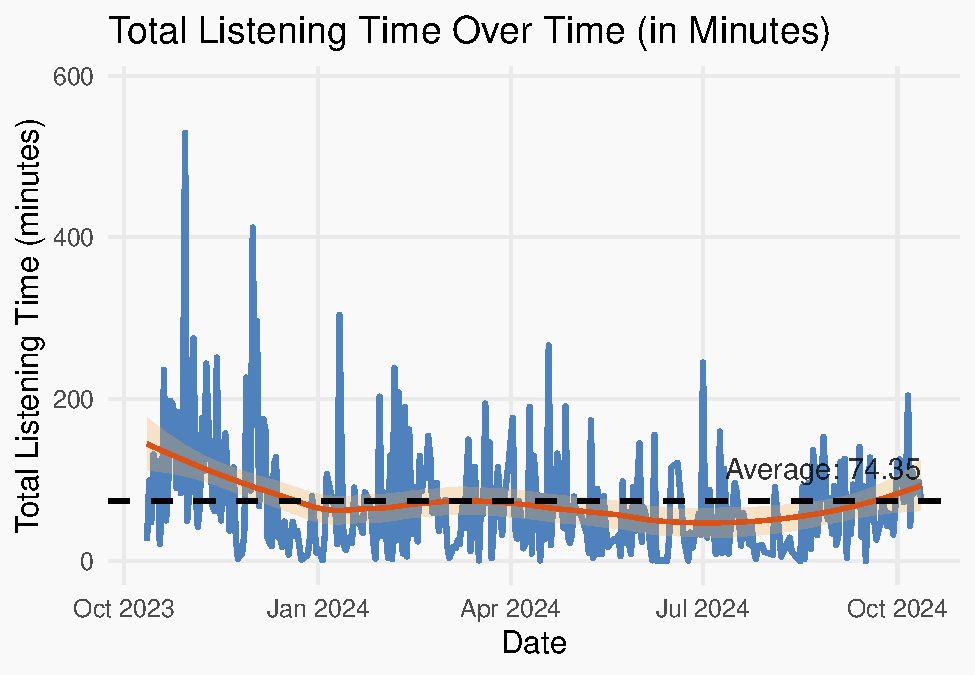
\includegraphics{SpotifyProjectPDF_files/figure-latex/unnamed-chunk-12-1.pdf}

\subsubsection{Top 15 Artists by Track
Engagement}\label{top-15-artists-by-track-engagement}

The bar plot showcases the top 15 artists based on total listening time,
measured in minutes. The x-axis represents the artist names, and the
y-axis indicates the total engagement, with bars showing the cumulative
time spent listening to each artist. The chart is oriented horizontally
to improve readability, making it easier to compare engagement levels
across different artists. A consistent soft blue color is used to
maintain a clean and visually appealing design.

From this plot, we can gain insights into listening preferences by
identifying the most frequently played artists. Artists with the longest
bars represent those with the highest engagement, suggesting that their
music resonates more or is preferred by the user. This information can
reveal patterns in music taste, highlight favorite genres or artists,
and help understand which musicians drive the most significant portion
of listening activity. It can also serve as a basis for personalized
recommendations or further exploration into why these particular artists
stand out.

\begin{Shaded}
\begin{Highlighting}[]
\FunctionTok{library}\NormalTok{(ggplot2)}
\FunctionTok{library}\NormalTok{(dplyr)}

\CommentTok{\# Aggregate total listening time by artist and convert msPlayed to minutes}
\NormalTok{artist\_engagement }\OtherTok{\textless{}{-}}\NormalTok{ combined\_data }\SpecialCharTok{\%\textgreater{}\%}
  \FunctionTok{group\_by}\NormalTok{(artistName) }\SpecialCharTok{\%\textgreater{}\%}
  \FunctionTok{summarise}\NormalTok{(}\AttributeTok{Total\_msPlayed =} \FunctionTok{sum}\NormalTok{(msPlayed) }\SpecialCharTok{/} \DecValTok{60000}\NormalTok{) }\SpecialCharTok{\%\textgreater{}\%}  \CommentTok{\# Convert to minutes}
  \FunctionTok{arrange}\NormalTok{(}\FunctionTok{desc}\NormalTok{(Total\_msPlayed)) }\SpecialCharTok{\%\textgreater{}\%}  \CommentTok{\# Sort artists by total listening time}
  \FunctionTok{slice\_head}\NormalTok{(}\AttributeTok{n =} \DecValTok{15}\NormalTok{)  }\CommentTok{\# Select top 15 artists}

\CommentTok{\# Create the bar plot}
\FunctionTok{ggplot}\NormalTok{(artist\_engagement, }\FunctionTok{aes}\NormalTok{(}\AttributeTok{x =} \FunctionTok{reorder}\NormalTok{(artistName, Total\_msPlayed), }\AttributeTok{y =}\NormalTok{ Total\_msPlayed)) }\SpecialCharTok{+}
  \FunctionTok{geom\_bar}\NormalTok{(}\AttributeTok{stat =} \StringTok{"identity"}\NormalTok{, }\AttributeTok{fill =} \StringTok{"\#4F81BD"}\NormalTok{) }\SpecialCharTok{+}  \CommentTok{\# Soft blue color for bars}
  \FunctionTok{coord\_flip}\NormalTok{() }\SpecialCharTok{+}  \CommentTok{\# Flip coordinates for better readability}
  \FunctionTok{labs}\NormalTok{(}\AttributeTok{title =} \StringTok{"Top 15 Artists by Track Engagement"}\NormalTok{,}
       \AttributeTok{x =} \StringTok{"Artist Name"}\NormalTok{, }\AttributeTok{y =} \StringTok{"Total Listening Time (minutes)"}\NormalTok{) }\SpecialCharTok{+}
  \FunctionTok{theme\_minimal}\NormalTok{(}\AttributeTok{base\_size =} \DecValTok{15}\NormalTok{) }\SpecialCharTok{+}  \CommentTok{\# Increase base font size for readability}
  \FunctionTok{theme}\NormalTok{(}\AttributeTok{panel.grid.major =} \FunctionTok{element\_line}\NormalTok{(}\AttributeTok{color =} \StringTok{"\#EAEAEA"}\NormalTok{),  }\CommentTok{\# Light grid lines}
        \AttributeTok{panel.grid.minor =} \FunctionTok{element\_blank}\NormalTok{(),  }\CommentTok{\# No minor grid lines}
        \AttributeTok{plot.background =} \FunctionTok{element\_rect}\NormalTok{(}\AttributeTok{fill =} \StringTok{"\#F9F9F9"}\NormalTok{, }\AttributeTok{color =} \ConstantTok{NA}\NormalTok{),  }\CommentTok{\# Soft background}
        \AttributeTok{legend.position =} \StringTok{"none"}\NormalTok{)  }\CommentTok{\# Remove legend if not needed}
\end{Highlighting}
\end{Shaded}

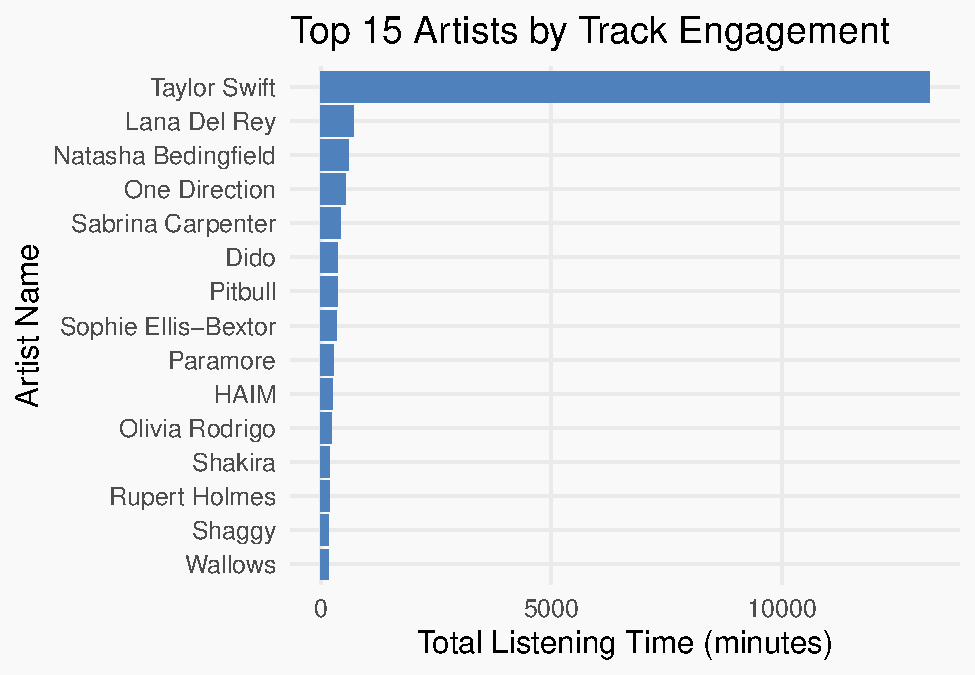
\includegraphics{SpotifyProjectPDF_files/figure-latex/unnamed-chunk-13-1.pdf}

\subsubsection{Mood Correlations with Danceability, Energy, and
Valence}\label{mood-correlations-with-danceability-energy-and-valence}

This analysis presents three 2D scatter plots that explore the
relationships between the musical features of danceability, energy, and
valence, while also considering the mood associated with each track. The
first scatter plot illustrates the correlation between danceability and
energy, providing insights into how these two features interact and
affect the overall mood of the music. The second plot examines the
relationship between danceability and valence, revealing how the rhythm
and tempo of a track relate to its emotional tone. Lastly, the third
plot analyzes energy against valence, further expanding our
understanding of how the intensity and emotional quality of music
influence listener mood. Each plot is color-coded according to mood
categories, making it easier to identify patterns and trends within the
dataset.

The scatter plots offer valuable insights into how specific musical
attributes align with different moods. For example, tracks characterized
by high danceability and energy may correlate with more upbeat and happy
moods, while tracks with lower energy but higher valence might represent
a more relaxed or melancholic state. The visual representation allows
for easy identification of clusters where certain moods are
concentrated, indicating a preference for particular musical qualities.
This understanding can help in creating more tailored music
recommendations based on mood, enhancing the listener's experience by
aligning their emotional state with the most suitable tracks. Moreover,
examining the relationships among these features could inform artists
and producers about the musical elements that resonate most with
audiences, guiding the creation of future music that better aligns with
listeners' emotional needs and preferences.

Ultimately, these plots not only serve as a means to visualize data but
also provide a deeper understanding of the interplay between music and
emotion, emphasizing how various musical characteristics can evoke or
reflect different moods in listeners. This exploration lays the
groundwork for further analysis and potential applications, such as
developing mood-based playlists or music recommendation systems that
leverage these insights to enhance user engagement and satisfaction.

\begin{Shaded}
\begin{Highlighting}[]
\CommentTok{\# Load necessary libraries without displaying messages}
\FunctionTok{suppressPackageStartupMessages}\NormalTok{(}\FunctionTok{library}\NormalTok{(dplyr))}
\FunctionTok{suppressPackageStartupMessages}\NormalTok{(}\FunctionTok{library}\NormalTok{(ggplot2))}

\CommentTok{\# Step 1: Data Preparation}
\CommentTok{\# Select relevant features and ensure mood labels are assigned}
\NormalTok{mood\_data }\OtherTok{\textless{}{-}}\NormalTok{ combined\_data }\SpecialCharTok{\%\textgreater{}\%}
  \FunctionTok{select}\NormalTok{(artistName, trackName, danceability, energy, valence, mood) }\SpecialCharTok{\%\textgreater{}\%}
  \FunctionTok{filter}\NormalTok{(}\SpecialCharTok{!}\FunctionTok{is.na}\NormalTok{(mood)) }\SpecialCharTok{\%\textgreater{}\%}
  \FunctionTok{na.omit}\NormalTok{()  }\CommentTok{\# Remove any additional rows with NA values}

\CommentTok{\# Group by artist and track to ensure multiple plays are considered}
\NormalTok{mood\_data }\OtherTok{\textless{}{-}}\NormalTok{ mood\_data }\SpecialCharTok{\%\textgreater{}\%}
  \FunctionTok{group\_by}\NormalTok{(artistName, trackName) }\SpecialCharTok{\%\textgreater{}\%}
  \FunctionTok{summarise}\NormalTok{(}\FunctionTok{across}\NormalTok{(}\FunctionTok{c}\NormalTok{(danceability, energy, valence), mean, }\AttributeTok{.names =} \StringTok{"avg\_\{col\}"}\NormalTok{),}
            \AttributeTok{mood =} \FunctionTok{first}\NormalTok{(mood),}
            \AttributeTok{.groups =} \StringTok{\textquotesingle{}drop\textquotesingle{}}\NormalTok{)}

\CommentTok{\# Define a custom color palette with more colors}
\NormalTok{custom\_colors }\OtherTok{\textless{}{-}} \FunctionTok{c}\NormalTok{(}\StringTok{\textquotesingle{}\#1f77b4\textquotesingle{}}\NormalTok{, }\StringTok{\textquotesingle{}\#ff7f0e\textquotesingle{}}\NormalTok{, }\StringTok{\textquotesingle{}\#2ca02c\textquotesingle{}}\NormalTok{, }\StringTok{\textquotesingle{}\#d62728\textquotesingle{}}\NormalTok{, }\StringTok{\textquotesingle{}\#9467bd\textquotesingle{}}\NormalTok{, }\StringTok{\textquotesingle{}\#8c564b\textquotesingle{}}\NormalTok{, }
                   \StringTok{\textquotesingle{}\#e377c2\textquotesingle{}}\NormalTok{, }\StringTok{\textquotesingle{}\#7f7f7f\textquotesingle{}}\NormalTok{, }\StringTok{\textquotesingle{}\#bcbd22\textquotesingle{}}\NormalTok{, }\StringTok{\textquotesingle{}\#17becf\textquotesingle{}}\NormalTok{, }\StringTok{\textquotesingle{}\#9edae5\textquotesingle{}}\NormalTok{, }\StringTok{\textquotesingle{}\#f7b6d2\textquotesingle{}}\NormalTok{, }
                   \StringTok{\textquotesingle{}\#d9d9d9\textquotesingle{}}\NormalTok{, }\StringTok{\textquotesingle{}\#ff9896\textquotesingle{}}\NormalTok{)}

\CommentTok{\# Step 2: Create 2D Scatter Plots separately using ggplot2}

\CommentTok{\# Scatter plot for Danceability vs. Energy}
\NormalTok{p1 }\OtherTok{\textless{}{-}} \FunctionTok{ggplot}\NormalTok{(mood\_data, }\FunctionTok{aes}\NormalTok{(}\AttributeTok{x =}\NormalTok{ avg\_danceability, }\AttributeTok{y =}\NormalTok{ avg\_energy, }\AttributeTok{color =}\NormalTok{ mood)) }\SpecialCharTok{+}
  \FunctionTok{geom\_point}\NormalTok{(}\AttributeTok{size =} \DecValTok{3}\NormalTok{, }\AttributeTok{alpha =} \FloatTok{0.8}\NormalTok{) }\SpecialCharTok{+}
  \FunctionTok{labs}\NormalTok{(}\AttributeTok{title =} \StringTok{"Danceability vs Energy"}\NormalTok{,}
       \AttributeTok{x =} \StringTok{"Danceability"}\NormalTok{,}
       \AttributeTok{y =} \StringTok{"Energy"}\NormalTok{) }\SpecialCharTok{+}
  \FunctionTok{theme\_minimal}\NormalTok{() }\SpecialCharTok{+}
  \FunctionTok{scale\_color\_manual}\NormalTok{(}\AttributeTok{values =}\NormalTok{ custom\_colors)}

\CommentTok{\# Scatter plot for Danceability vs. Valence}
\NormalTok{p2 }\OtherTok{\textless{}{-}} \FunctionTok{ggplot}\NormalTok{(mood\_data, }\FunctionTok{aes}\NormalTok{(}\AttributeTok{x =}\NormalTok{ avg\_danceability, }\AttributeTok{y =}\NormalTok{ avg\_valence, }\AttributeTok{color =}\NormalTok{ mood)) }\SpecialCharTok{+}
  \FunctionTok{geom\_point}\NormalTok{(}\AttributeTok{size =} \DecValTok{3}\NormalTok{, }\AttributeTok{alpha =} \FloatTok{0.8}\NormalTok{) }\SpecialCharTok{+}
  \FunctionTok{labs}\NormalTok{(}\AttributeTok{title =} \StringTok{"Danceability vs Valence"}\NormalTok{,}
       \AttributeTok{x =} \StringTok{"Danceability"}\NormalTok{,}
       \AttributeTok{y =} \StringTok{"Valence"}\NormalTok{) }\SpecialCharTok{+}
  \FunctionTok{theme\_minimal}\NormalTok{() }\SpecialCharTok{+}
  \FunctionTok{scale\_color\_manual}\NormalTok{(}\AttributeTok{values =}\NormalTok{ custom\_colors)}

\CommentTok{\# Scatter plot for Energy vs. Valence}
\NormalTok{p3 }\OtherTok{\textless{}{-}} \FunctionTok{ggplot}\NormalTok{(mood\_data, }\FunctionTok{aes}\NormalTok{(}\AttributeTok{x =}\NormalTok{ avg\_energy, }\AttributeTok{y =}\NormalTok{ avg\_valence, }\AttributeTok{color =}\NormalTok{ mood)) }\SpecialCharTok{+}
  \FunctionTok{geom\_point}\NormalTok{(}\AttributeTok{size =} \DecValTok{3}\NormalTok{, }\AttributeTok{alpha =} \FloatTok{0.8}\NormalTok{) }\SpecialCharTok{+}
  \FunctionTok{labs}\NormalTok{(}\AttributeTok{title =} \StringTok{"Energy vs Valence"}\NormalTok{,}
       \AttributeTok{x =} \StringTok{"Energy"}\NormalTok{,}
       \AttributeTok{y =} \StringTok{"Valence"}\NormalTok{) }\SpecialCharTok{+}
  \FunctionTok{theme\_minimal}\NormalTok{() }\SpecialCharTok{+}
  \FunctionTok{scale\_color\_manual}\NormalTok{(}\AttributeTok{values =}\NormalTok{ custom\_colors)}

\CommentTok{\# Show the plots}
\FunctionTok{print}\NormalTok{(p1)}
\end{Highlighting}
\end{Shaded}

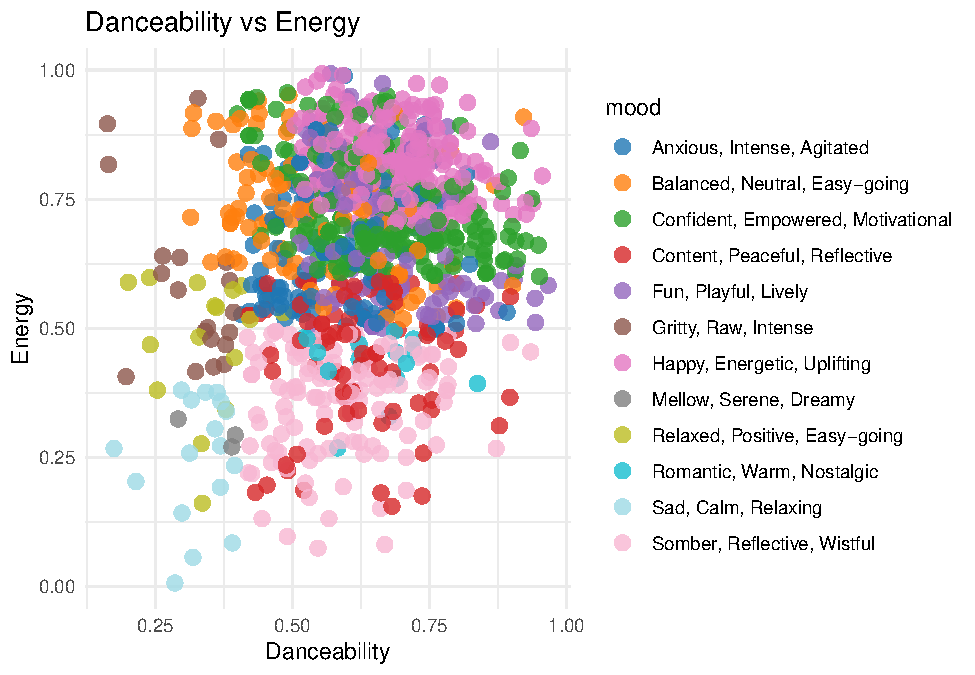
\includegraphics{SpotifyProjectPDF_files/figure-latex/unnamed-chunk-14-1.pdf}

\begin{Shaded}
\begin{Highlighting}[]
\FunctionTok{print}\NormalTok{(p2)}
\end{Highlighting}
\end{Shaded}

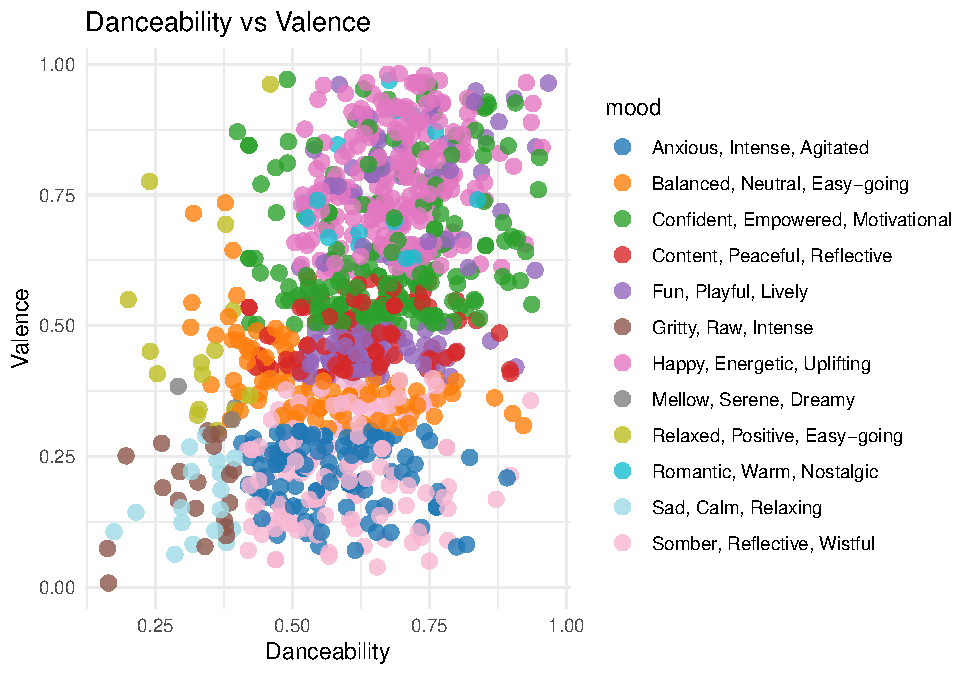
\includegraphics{SpotifyProjectPDF_files/figure-latex/unnamed-chunk-14-2.pdf}

\begin{Shaded}
\begin{Highlighting}[]
\FunctionTok{print}\NormalTok{(p3)}
\end{Highlighting}
\end{Shaded}

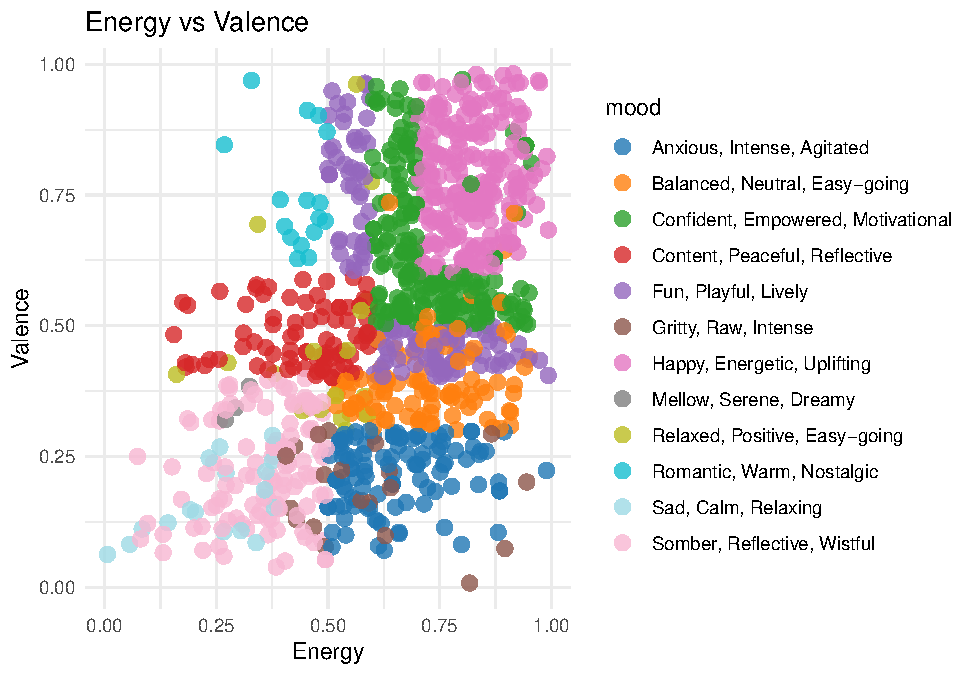
\includegraphics{SpotifyProjectPDF_files/figure-latex/unnamed-chunk-14-3.pdf}

\subsubsection{Normalized Listening Time for Top 5 Artists Over
Time}\label{normalized-listening-time-for-top-5-artists-over-time}

This analysis focuses on visualizing the normalized listening time for
the top five artists based on total listening duration. The dataset is
first prepared by converting the listening time from milliseconds to
minutes, then aggregating the total listening time per artist for each
date. The top five artists are identified based on their cumulative
listening time. To enable meaningful comparisons across different
artists, their listening times are normalized. Normalization is crucial
as it adjusts the data to a common scale, allowing for a direct
comparison of listening habits regardless of the absolute differences in
total listening times between artists. This means that the values
represent a proportion of each artist's maximum listening time, making
it easier to observe trends and patterns over time.

In this visualization, a moving average is applied to the normalized
listening times to smooth out short-term fluctuations and highlight
longer-term trends. The line chart, which displays the normalized
listening time of the top five artists over time, provides insights into
how listener engagement varies for each artist. The use of a custom
color palette enhances the readability of the chart, allowing viewers to
quickly identify trends for each artist. By representing normalized
listening times, the analysis reveals not just the popularity of each
artist, but also how their engagement levels change over time relative
to each other, offering valuable insights into listener preferences and
shifts in music consumption habits. This information can be particularly
useful for artists and producers aiming to understand their audience
better and tailor their marketing strategies accordingly.

Furthermore, the smoothing process helps mitigate the impact of outliers
or anomalies in daily listening behavior, thereby allowing for a clearer
view of consistent patterns. By focusing on normalized values, the chart
encourages a better understanding of listening dynamics among the top
artists, illuminating moments of increased popularity or decline that
may correlate with external factors such as new releases, media
coverage, or social trends. This nuanced approach fosters a
comprehensive analysis of listener engagement and can guide decisions
for future content creation or promotional efforts within the music
industry.

\begin{Shaded}
\begin{Highlighting}[]
\CommentTok{\# Load necessary libraries without displaying messages}
\FunctionTok{suppressPackageStartupMessages}\NormalTok{(}\FunctionTok{library}\NormalTok{(dplyr))}
\FunctionTok{suppressPackageStartupMessages}\NormalTok{(}\FunctionTok{library}\NormalTok{(ggplot2))}
\FunctionTok{suppressPackageStartupMessages}\NormalTok{(}\FunctionTok{library}\NormalTok{(lubridate))}
\FunctionTok{suppressPackageStartupMessages}\NormalTok{(}\FunctionTok{library}\NormalTok{(zoo))  }\CommentTok{\# For the rollmean function}

\CommentTok{\# Step 1: Data Preparation}
\CommentTok{\# Assume combined\_data has an \textquotesingle{}end\_time\textquotesingle{} column and \textquotesingle{}milliseconds\_played\textquotesingle{} for the listening time.}
\CommentTok{\# Convert end\_time to Date format if it\textquotesingle{}s not already}
\NormalTok{combined\_data}\SpecialCharTok{$}\NormalTok{endTime }\OtherTok{\textless{}{-}} \FunctionTok{as.Date}\NormalTok{(combined\_data}\SpecialCharTok{$}\NormalTok{endTime)}

\CommentTok{\# Convert milliseconds played to minutes}
\NormalTok{combined\_data}\SpecialCharTok{$}\NormalTok{minutes\_played }\OtherTok{\textless{}{-}}\NormalTok{ combined\_data}\SpecialCharTok{$}\NormalTok{msPlayed }\SpecialCharTok{/} \DecValTok{60000}  \CommentTok{\# Convert to minutes}

\CommentTok{\# Aggregate data to get total listening time in minutes for each artist over time}
\NormalTok{artist\_time\_data }\OtherTok{\textless{}{-}}\NormalTok{ combined\_data }\SpecialCharTok{\%\textgreater{}\%}
\NormalTok{  dplyr}\SpecialCharTok{::}\FunctionTok{group\_by}\NormalTok{(endTime, artistName) }\SpecialCharTok{\%\textgreater{}\%}
\NormalTok{  dplyr}\SpecialCharTok{::}\FunctionTok{summarise}\NormalTok{(}\AttributeTok{total\_minutes =} \FunctionTok{sum}\NormalTok{(minutes\_played), }\AttributeTok{.groups =} \StringTok{\textquotesingle{}drop\textquotesingle{}}\NormalTok{) }\SpecialCharTok{\%\textgreater{}\%}
\NormalTok{  dplyr}\SpecialCharTok{::}\FunctionTok{arrange}\NormalTok{(endTime)}

\CommentTok{\# Get the top 5 artists based on total listening time}
\NormalTok{top\_artists }\OtherTok{\textless{}{-}}\NormalTok{ artist\_time\_data }\SpecialCharTok{\%\textgreater{}\%}
\NormalTok{  dplyr}\SpecialCharTok{::}\FunctionTok{group\_by}\NormalTok{(artistName) }\SpecialCharTok{\%\textgreater{}\%}
\NormalTok{  dplyr}\SpecialCharTok{::}\FunctionTok{summarise}\NormalTok{(}\AttributeTok{total =} \FunctionTok{sum}\NormalTok{(total\_minutes)) }\SpecialCharTok{\%\textgreater{}\%}
\NormalTok{  dplyr}\SpecialCharTok{::}\FunctionTok{top\_n}\NormalTok{(}\DecValTok{5}\NormalTok{, total) }\SpecialCharTok{\%\textgreater{}\%}
\NormalTok{  dplyr}\SpecialCharTok{::}\FunctionTok{pull}\NormalTok{(artistName)}

\CommentTok{\# Filter the data to keep only top 5 artists}
\NormalTok{top\_artist\_time\_data }\OtherTok{\textless{}{-}}\NormalTok{ artist\_time\_data }\SpecialCharTok{\%\textgreater{}\%}
\NormalTok{  dplyr}\SpecialCharTok{::}\FunctionTok{filter}\NormalTok{(artistName }\SpecialCharTok{\%in\%}\NormalTok{ top\_artists)}

\CommentTok{\# Normalize the listening time for each artist}
\NormalTok{top\_artist\_time\_data }\OtherTok{\textless{}{-}}\NormalTok{ top\_artist\_time\_data }\SpecialCharTok{\%\textgreater{}\%}
\NormalTok{  dplyr}\SpecialCharTok{::}\FunctionTok{group\_by}\NormalTok{(artistName) }\SpecialCharTok{\%\textgreater{}\%}
\NormalTok{  dplyr}\SpecialCharTok{::}\FunctionTok{mutate}\NormalTok{(}\AttributeTok{normalized\_minutes =}\NormalTok{ total\_minutes }\SpecialCharTok{/} \FunctionTok{max}\NormalTok{(total\_minutes)) }\SpecialCharTok{\%\textgreater{}\%}
\NormalTok{  dplyr}\SpecialCharTok{::}\FunctionTok{ungroup}\NormalTok{()}

\CommentTok{\# Smooth the normalized\_minutes using a moving average and remove NAs}
\NormalTok{top\_artist\_time\_data }\OtherTok{\textless{}{-}}\NormalTok{ top\_artist\_time\_data }\SpecialCharTok{\%\textgreater{}\%}
\NormalTok{  dplyr}\SpecialCharTok{::}\FunctionTok{group\_by}\NormalTok{(artistName) }\SpecialCharTok{\%\textgreater{}\%}
\NormalTok{  dplyr}\SpecialCharTok{::}\FunctionTok{mutate}\NormalTok{(}\AttributeTok{smooth\_minutes =}\NormalTok{ zoo}\SpecialCharTok{::}\FunctionTok{rollmean}\NormalTok{(normalized\_minutes, }\AttributeTok{k =} \DecValTok{7}\NormalTok{, }\AttributeTok{fill =} \ConstantTok{NA}\NormalTok{, }\AttributeTok{align =} \StringTok{"right"}\NormalTok{)) }\SpecialCharTok{\%\textgreater{}\%}
\NormalTok{  dplyr}\SpecialCharTok{::}\FunctionTok{ungroup}\NormalTok{() }\SpecialCharTok{\%\textgreater{}\%}
\NormalTok{  dplyr}\SpecialCharTok{::}\FunctionTok{filter}\NormalTok{(}\SpecialCharTok{!}\FunctionTok{is.na}\NormalTok{(smooth\_minutes))  }\CommentTok{\# Remove NAs}

\CommentTok{\# Define a custom color palette with more colors}
\NormalTok{custom\_colors }\OtherTok{\textless{}{-}} \FunctionTok{c}\NormalTok{(}\StringTok{\textquotesingle{}\#ff7f0e\textquotesingle{}}\NormalTok{, }\StringTok{\textquotesingle{}\#1f77b4\textquotesingle{}}\NormalTok{, }\StringTok{\textquotesingle{}\#2ca02c\textquotesingle{}}\NormalTok{, }\StringTok{\textquotesingle{}\#d62728\textquotesingle{}}\NormalTok{, }\StringTok{\textquotesingle{}\#9467bd\textquotesingle{}}\NormalTok{, }\StringTok{\textquotesingle{}\#8c564b\textquotesingle{}}\NormalTok{, }
                   \StringTok{\textquotesingle{}\#e377c2\textquotesingle{}}\NormalTok{, }\StringTok{\textquotesingle{}\#7f7f7f\textquotesingle{}}\NormalTok{, }\StringTok{\textquotesingle{}\#bcbd22\textquotesingle{}}\NormalTok{, }\StringTok{\textquotesingle{}\#17becf\textquotesingle{}}\NormalTok{, }\StringTok{\textquotesingle{}\#9edae5\textquotesingle{}}\NormalTok{, }\StringTok{\textquotesingle{}\#f7b6d2\textquotesingle{}}\NormalTok{)}

\CommentTok{\# Create Line Chart for Top 5 Artists Over Time using ggplot2}
\NormalTok{line\_chart }\OtherTok{\textless{}{-}} \FunctionTok{ggplot}\NormalTok{(top\_artist\_time\_data, }\FunctionTok{aes}\NormalTok{(}\AttributeTok{x =}\NormalTok{ endTime, }\AttributeTok{y =}\NormalTok{ smooth\_minutes, }\AttributeTok{color =}\NormalTok{ artistName)) }\SpecialCharTok{+}
  \FunctionTok{geom\_line}\NormalTok{(}\AttributeTok{size =} \DecValTok{1}\NormalTok{) }\SpecialCharTok{+}
  \FunctionTok{labs}\NormalTok{(}\AttributeTok{title =} \StringTok{"Normalized Listening Time for Top 5 Artists Over Time"}\NormalTok{,}
       \AttributeTok{x =} \StringTok{"Date"}\NormalTok{,}
       \AttributeTok{y =} \StringTok{"Normalized Listening Time"}\NormalTok{) }\SpecialCharTok{+}
  \FunctionTok{theme\_minimal}\NormalTok{() }\SpecialCharTok{+}
  \FunctionTok{scale\_color\_manual}\NormalTok{(}\AttributeTok{values =}\NormalTok{ custom\_colors)}
\end{Highlighting}
\end{Shaded}

\begin{verbatim}
## Warning: Using `size` aesthetic for lines was deprecated in ggplot2 3.4.0.
## i Please use `linewidth` instead.
## This warning is displayed once every 8 hours.
## Call `lifecycle::last_lifecycle_warnings()` to see where this warning was
## generated.
\end{verbatim}

\begin{Shaded}
\begin{Highlighting}[]
\CommentTok{\# Print the line chart}
\FunctionTok{print}\NormalTok{(line\_chart)}
\end{Highlighting}
\end{Shaded}

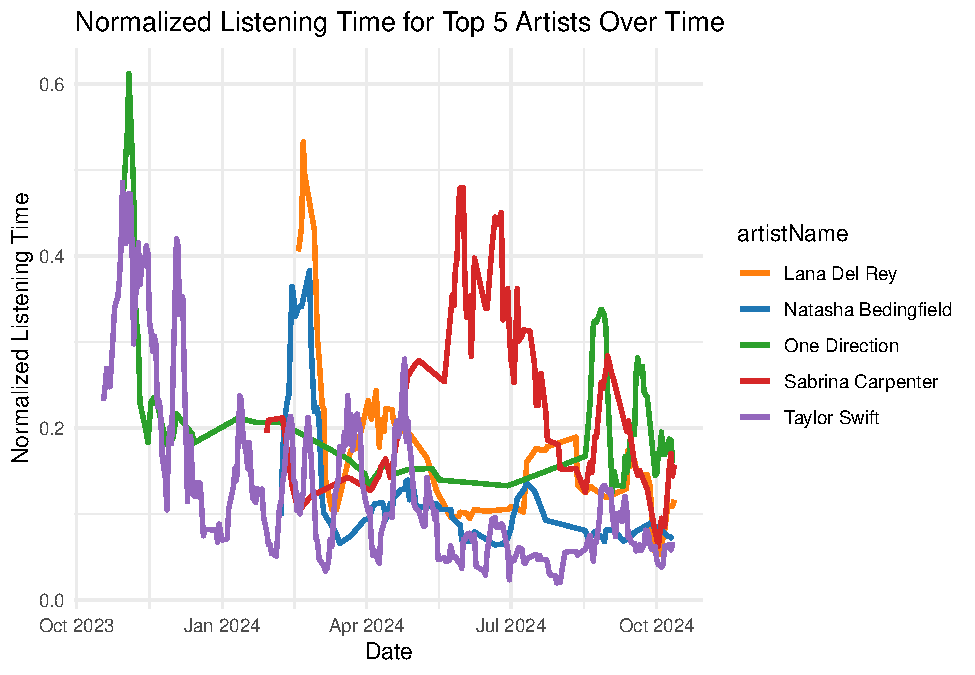
\includegraphics{SpotifyProjectPDF_files/figure-latex/unnamed-chunk-15-1.pdf}

\subsubsection{Mood Distribution by Day of the
Week}\label{mood-distribution-by-day-of-the-week}

This analysis examines how listeners' moods vary throughout the week,
providing insights into potential trends in music consumption based on
emotional states. The first step involves preparing the data by
converting the endTime column to a date format and extracting the day of
the week from these dates. This allows for a categorical analysis of
moods across different days, facilitating a clearer understanding of how
mood distribution may fluctuate in relation to the weekly cycle.

Next, the mood distribution is summarized by counting occurrences of
each mood for each day of the week. This summary includes a calculation
of the percentage of each mood relative to the total number of entries
for that day, enabling a normalized view of mood representation. By
filtering out any missing mood values, the analysis ensures that only
complete cases are considered, providing a more accurate portrayal of
the data.

The visualization employs a stacked bar chart to represent the mood
distribution, where each bar corresponds to a day of the week, and the
segments within each bar indicate the proportion of different moods.
This method highlights not only the predominant moods for each day but
also how they compare across the week. The use of the ``Set3'' color
palette from the scale\_fill\_brewer function enhances the readability
of the chart, ensuring that different moods are easily distinguishable.
By visualizing the mood distribution in this manner, the analysis sheds
light on patterns in listener emotions and how they might correlate with
specific days, which can be particularly useful for understanding the
psychological aspects of music consumption and for tailoring music
recommendations or playlists based on the day of the week.

\begin{Shaded}
\begin{Highlighting}[]
\CommentTok{\# Load necessary libraries}
\FunctionTok{library}\NormalTok{(dplyr)}
\FunctionTok{library}\NormalTok{(ggplot2)}

\CommentTok{\# Step 1: Data Preparation}
\CommentTok{\# Assume combined\_data has an \textquotesingle{}endTime\textquotesingle{} column and \textquotesingle{}mood\textquotesingle{} column.}

\CommentTok{\# Convert endTime to Date format if it\textquotesingle{}s not already}
\NormalTok{combined\_data}\SpecialCharTok{$}\NormalTok{endTime }\OtherTok{\textless{}{-}} \FunctionTok{as.Date}\NormalTok{(combined\_data}\SpecialCharTok{$}\NormalTok{endTime)}

\CommentTok{\# Add a new column for the day of the week}
\NormalTok{combined\_data}\SpecialCharTok{$}\NormalTok{day\_of\_week }\OtherTok{\textless{}{-}} \FunctionTok{weekdays}\NormalTok{(combined\_data}\SpecialCharTok{$}\NormalTok{endTime)}

\CommentTok{\# Step 2: Summarize mood distribution by day of the week}
\NormalTok{mood\_distribution }\OtherTok{\textless{}{-}}\NormalTok{ combined\_data }\SpecialCharTok{\%\textgreater{}\%}
  \FunctionTok{select}\NormalTok{(day\_of\_week, mood) }\SpecialCharTok{\%\textgreater{}\%}
  \FunctionTok{filter}\NormalTok{(}\SpecialCharTok{!}\FunctionTok{is.na}\NormalTok{(mood)) }\SpecialCharTok{\%\textgreater{}\%}
  \FunctionTok{count}\NormalTok{(day\_of\_week, mood) }\SpecialCharTok{\%\textgreater{}\%}
  \FunctionTok{group\_by}\NormalTok{(day\_of\_week) }\SpecialCharTok{\%\textgreater{}\%}
  \FunctionTok{mutate}\NormalTok{(}\AttributeTok{percentage =}\NormalTok{ n }\SpecialCharTok{/} \FunctionTok{sum}\NormalTok{(n) }\SpecialCharTok{*} \DecValTok{100}\NormalTok{)}

\CommentTok{\# Step 3: Plot the mood distribution by day of the week}
\FunctionTok{ggplot}\NormalTok{(mood\_distribution, }\FunctionTok{aes}\NormalTok{(}\AttributeTok{x =}\NormalTok{ day\_of\_week, }\AttributeTok{y =}\NormalTok{ percentage, }\AttributeTok{fill =}\NormalTok{ mood)) }\SpecialCharTok{+}
  \FunctionTok{geom\_bar}\NormalTok{(}\AttributeTok{stat =} \StringTok{"identity"}\NormalTok{, }\AttributeTok{position =} \StringTok{"fill"}\NormalTok{) }\SpecialCharTok{+}
  \FunctionTok{labs}\NormalTok{(}\AttributeTok{title =} \StringTok{"Mood Distribution by Day of the Week"}\NormalTok{,}
       \AttributeTok{x =} \StringTok{"Day of the Week"}\NormalTok{,}
       \AttributeTok{y =} \StringTok{"Percentage"}\NormalTok{,}
       \AttributeTok{fill =} \StringTok{"Mood"}\NormalTok{) }\SpecialCharTok{+}
  \FunctionTok{theme\_minimal}\NormalTok{() }\SpecialCharTok{+}
  \FunctionTok{scale\_fill\_brewer}\NormalTok{(}\AttributeTok{palette =} \StringTok{"Set3"}\NormalTok{)  }\CommentTok{\# Choose a suitable color palette}
\end{Highlighting}
\end{Shaded}

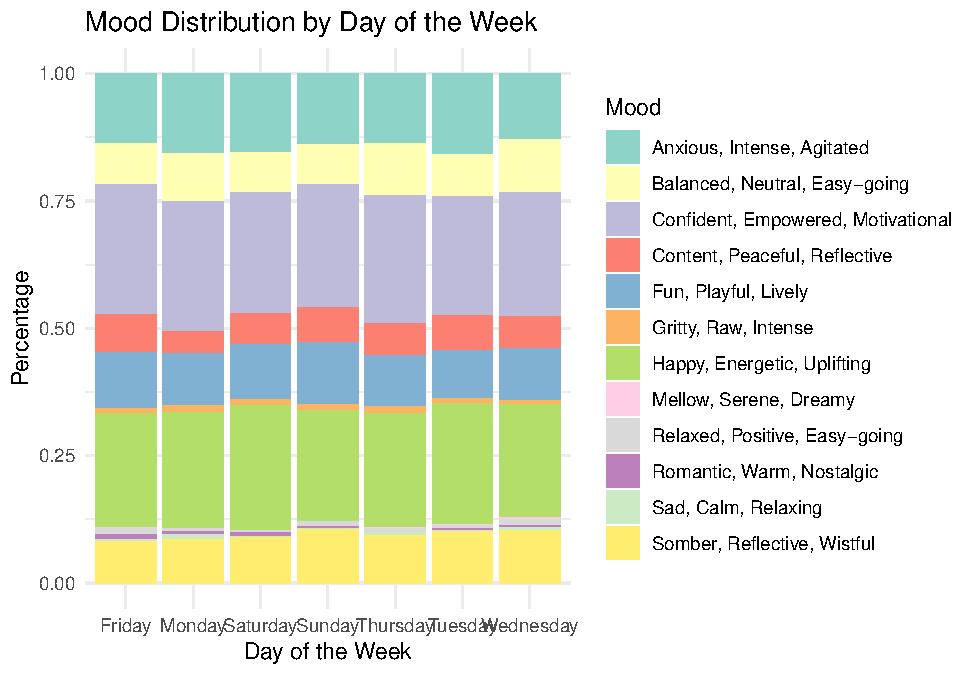
\includegraphics{SpotifyProjectPDF_files/figure-latex/unnamed-chunk-16-1.pdf}

\subsubsection{Conclusion of the Data Visualization
Section}\label{conclusion-of-the-data-visualization-section}

The data visualization section of the analysis highlights significant
insights into the emotional dynamics of music consumption through
various visual representations. By utilizing scatter plots, we examined
the relationships between key audio features---danceability, energy, and
valence---and how they correspond to different mood classifications. The
findings suggest clear trends in how these attributes interplay,
offering a nuanced understanding of listener preferences and emotional
responses.

Furthermore, the line charts depicting normalized listening times for
the top artists over time revealed patterns in engagement and
popularity, demonstrating how listener habits fluctuate across different
periods. These visualizations not only enhance the interpretability of
the data but also facilitate deeper insights into user behavior,
informing future music recommendations and targeted engagement
strategies.

Overall, this section underscores the importance of effective data
visualization in deriving actionable conclusions from complex datasets,
allowing for a richer understanding of the multifaceted relationships
between music characteristics and listener emotions.

\subsection{Part 5: Music Recommendation System based on user
mood}\label{part-5-music-recommendation-system-based-on-user-mood}

In today's digital age, music streaming services provide vast libraries
of songs, making it essential to develop personalized recommendation
systems that enhance user experience. This section outlines the
methodology used to create a personalized music recommendation system
based on user preferences, including mood, favorite artists, and
disliked artists. The system utilizes a dataset of listening habits and
audio features to generate tailored song recommendations.

\subsubsection{Methodology}\label{methodology-1}

\begin{enumerate}
\def\labelenumi{\arabic{enumi}.}
\item
  \textbf{Data Loading}: The first step involves loading the dataset
  containing music information, including artist names, track names,
  mood indicators, and user listening habits. The read\_csv function
  from the readr library is utilized to import the data efficiently
  while suppressing type messages for a cleaner output.
\item
  \textbf{User Profile Creation}: A user profile is constructed to
  encapsulate the individual's preferences. This profile includes:

  \begin{itemize}
  \item
    \textbf{Preferred Moods}: The moods that the user enjoys in music,
    such as ``Happy,'' ``Energetic,'' ``Uplifting,'' ``Confident,''
    ``Empowered,'' and ``Motivational.''
  \item
    \textbf{Favorite Artists}: A list of artists the user particularly
    enjoys, e.g., ``Taylor Swift'' and ``JAY-Z.''
  \item
    \textbf{Disliked Artists}: Artists that the user prefers to avoid,
    e.g., ``Kenya Grace.''
  \end{itemize}
\item
  \textbf{Recommendation Function}: A dedicated function,
  recommend\_songs\_personalized, processes the user profile and dataset
  to generate song recommendations. The function operates as follows:

  \begin{itemize}
  \item
    \textbf{Initialize Recommendations}: It starts by creating an empty
    data frame to store the recommended songs.
  \item
    \textbf{Mood-Based Filtering}: The function iterates through the
    user's preferred moods. For each mood, it filters the dataset to
    find songs that match the mood criteria, using the str\_detect
    function to ensure case-insensitive matching. The filtered results
    are appended to the recommendations data frame.
  \item
    \textbf{Disliked Artists Filtering}: After gathering mood-based
    recommendations, the function checks for any disliked artists
    specified in the user profile. It removes any recommendations that
    include these artists.
  \item
    \textbf{Favorite Artists Inclusion}: The function then looks for
    songs by the user's favorite artists and adds them to the
    recommendations list.
  \item
    \textbf{Finalizing Recommendations}: Duplicates are removed from the
    recommendations, and a random sample of songs is selected based on
    the number specified (defaulting to 10). This ensures variety in the
    recommendations.
  \end{itemize}
\item
  \textbf{Displaying Recommendations}: Finally, the system checks
  whether any recommendations were generated. If there are results, they
  are formatted into a visually appealing table using the kable and
  kableExtra libraries. This enhances readability, making it easier for
  users to explore their personalized music options.
\end{enumerate}

\subsubsection{Benefits of the
Methodology}\label{benefits-of-the-methodology}

\begin{itemize}
\item
  \textbf{Personalization}: By considering individual preferences for
  mood, favorite artists, and dislikes, the recommendation system
  provides a more relevant and enjoyable listening experience.
\item
  \textbf{Flexibility}: The system allows for easy updates to the user
  profile, enabling dynamic recommendations that can adapt to changing
  musical tastes.
\item
  \textbf{User Engagement}: Presenting recommendations in an organized
  and aesthetically pleasing format encourages users to explore new
  music, increasing overall engagement with the platform.
\item
  \textbf{Scalability}: The methodology can be applied to larger
  datasets and expanded to include more complex recommendation
  algorithms, such as collaborative filtering or machine learning
  techniques.
\end{itemize}

In summary, this personalized music recommendation system not only
enhances user satisfaction but also fosters a deeper connection to music
by catering to individual preferences and moods.

\begin{Shaded}
\begin{Highlighting}[]
\CommentTok{\# Load necessary libraries}
\FunctionTok{library}\NormalTok{(dplyr)}
\FunctionTok{library}\NormalTok{(readr)}
\FunctionTok{library}\NormalTok{(knitr)}
\FunctionTok{library}\NormalTok{(kableExtra)}
\FunctionTok{library}\NormalTok{(stringr)}

\CommentTok{\# Step 1: Load the combined data}
\NormalTok{combined\_data }\OtherTok{\textless{}{-}} \FunctionTok{read\_csv}\NormalTok{(}\StringTok{"combined\_data.csv"}\NormalTok{, }\AttributeTok{show\_col\_types =} \ConstantTok{FALSE}\NormalTok{)}

\CommentTok{\# Step 2: Create a user profile}
\NormalTok{user\_profile }\OtherTok{\textless{}{-}} \FunctionTok{list}\NormalTok{(}
  \AttributeTok{preferred\_moods =} \FunctionTok{c}\NormalTok{(}\StringTok{"Happy, Energetic, Uplifting"}\NormalTok{, }\StringTok{"Confident, Empowered, Motivational"}\NormalTok{),}
  \AttributeTok{favorite\_artists =} \FunctionTok{c}\NormalTok{(}\StringTok{"Taylor Swift"}\NormalTok{, }\StringTok{"JAY{-}Z"}\NormalTok{),}
  \AttributeTok{disliked\_artists =} \FunctionTok{c}\NormalTok{(}\StringTok{"Kenya Grace"}\NormalTok{)}
\NormalTok{)}

\CommentTok{\# Step 3: Function to recommend songs based on user profile}
\NormalTok{recommend\_songs\_personalized }\OtherTok{\textless{}{-}} \ControlFlowTok{function}\NormalTok{(user\_profile, data, }\AttributeTok{num\_recommendations =} \DecValTok{10}\NormalTok{) \{}
  \CommentTok{\# Initialize an empty data frame for recommendations}
\NormalTok{  recommendations }\OtherTok{\textless{}{-}} \FunctionTok{data.frame}\NormalTok{(}\AttributeTok{artistName=}\FunctionTok{character}\NormalTok{(), }\AttributeTok{trackName=}\FunctionTok{character}\NormalTok{(), }\AttributeTok{mood=}\FunctionTok{character}\NormalTok{(), }\AttributeTok{stringsAsFactors=}\ConstantTok{FALSE}\NormalTok{)}
  
  \CommentTok{\# Filter based on preferred moods}
  \ControlFlowTok{for}\NormalTok{ (mood }\ControlFlowTok{in}\NormalTok{ user\_profile}\SpecialCharTok{$}\NormalTok{preferred\_moods) \{}
\NormalTok{    mood\_recommendations }\OtherTok{\textless{}{-}}\NormalTok{ data }\SpecialCharTok{\%\textgreater{}\%}
      \FunctionTok{filter}\NormalTok{(}\FunctionTok{str\_detect}\NormalTok{(}\FunctionTok{tolower}\NormalTok{(mood), }\FunctionTok{tolower}\NormalTok{(}\FunctionTok{trimws}\NormalTok{(mood)))) }\SpecialCharTok{\%\textgreater{}\%}
      \FunctionTok{select}\NormalTok{(artistName, trackName, mood) }\SpecialCharTok{\%\textgreater{}\%}
      \FunctionTok{distinct}\NormalTok{()}
\NormalTok{    recommendations }\OtherTok{\textless{}{-}} \FunctionTok{rbind}\NormalTok{(recommendations, mood\_recommendations)}
\NormalTok{  \}}
  
  \CommentTok{\# Filter out disliked artists}
  \ControlFlowTok{if}\NormalTok{ (}\SpecialCharTok{!}\FunctionTok{is.null}\NormalTok{(user\_profile}\SpecialCharTok{$}\NormalTok{disliked\_artists)) \{}
\NormalTok{    recommendations }\OtherTok{\textless{}{-}}\NormalTok{ recommendations }\SpecialCharTok{\%\textgreater{}\%}
      \FunctionTok{filter}\NormalTok{(}\SpecialCharTok{!}\NormalTok{artistName }\SpecialCharTok{\%in\%}\NormalTok{ user\_profile}\SpecialCharTok{$}\NormalTok{disliked\_artists)}
\NormalTok{  \}}
  
  \CommentTok{\# Include favorite artists if specified}
  \ControlFlowTok{if}\NormalTok{ (}\SpecialCharTok{!}\FunctionTok{is.null}\NormalTok{(user\_profile}\SpecialCharTok{$}\NormalTok{favorite\_artists)) \{}
\NormalTok{    favorite\_recommendations }\OtherTok{\textless{}{-}}\NormalTok{ data }\SpecialCharTok{\%\textgreater{}\%}
      \FunctionTok{filter}\NormalTok{(artistName }\SpecialCharTok{\%in\%}\NormalTok{ user\_profile}\SpecialCharTok{$}\NormalTok{favorite\_artists) }\SpecialCharTok{\%\textgreater{}\%}
      \FunctionTok{select}\NormalTok{(artistName, trackName, mood) }\SpecialCharTok{\%\textgreater{}\%}
      \FunctionTok{distinct}\NormalTok{()}
\NormalTok{    recommendations }\OtherTok{\textless{}{-}} \FunctionTok{rbind}\NormalTok{(recommendations, favorite\_recommendations)}
\NormalTok{  \}}
  
  \CommentTok{\# Remove duplicates and sample recommendations}
\NormalTok{  recommendations }\OtherTok{\textless{}{-}}\NormalTok{ recommendations }\SpecialCharTok{\%\textgreater{}\%}
    \FunctionTok{distinct}\NormalTok{() }\SpecialCharTok{\%\textgreater{}\%}
    \FunctionTok{sample\_n}\NormalTok{(}\FunctionTok{min}\NormalTok{(num\_recommendations, }\FunctionTok{nrow}\NormalTok{(.)))}
  
  \FunctionTok{return}\NormalTok{(recommendations)}
\NormalTok{\}}

\CommentTok{\# Step 4: Get personalized recommendations}
\NormalTok{personalized\_recommendations }\OtherTok{\textless{}{-}} \FunctionTok{recommend\_songs\_personalized}\NormalTok{(user\_profile, combined\_data)}

\CommentTok{\# Step 5: Display personalized recommended songs}
\ControlFlowTok{if}\NormalTok{ (}\FunctionTok{nrow}\NormalTok{(personalized\_recommendations) }\SpecialCharTok{\textgreater{}} \DecValTok{0}\NormalTok{) \{}
\NormalTok{  personalized\_recommendations }\SpecialCharTok{\%\textgreater{}\%}
    \FunctionTok{kable}\NormalTok{() }\SpecialCharTok{\%\textgreater{}\%}
    \FunctionTok{kable\_styling}\NormalTok{(}\AttributeTok{bootstrap\_options =} \FunctionTok{c}\NormalTok{(}\StringTok{"striped"}\NormalTok{, }\StringTok{"hover"}\NormalTok{, }\StringTok{"condensed"}\NormalTok{))}
\NormalTok{\} }\ControlFlowTok{else}\NormalTok{ \{}
  \FunctionTok{print}\NormalTok{(}\StringTok{"No personalized recommendations could be found."}\NormalTok{)}
\NormalTok{\}}
\end{Highlighting}
\end{Shaded}

\begin{longtable}[t]{lll}
\toprule
artistName & trackName & mood\\
\midrule
Taylor Swift & End Game & Anxious, Intense, Agitated\\
Taylor Swift & Come In With The Rain (Taylor’s Version) & Anxious, Intense, Agitated\\
Calvin Harris & Pray to God (feat. HAIM) & Fun, Playful, Lively\\
Taylor Swift & Soon You’ll Get Better (feat. The Chicks) & Content, Peaceful, Reflective\\
Taylor Swift & Babe (Taylor's Version) (From The Vault) & Happy, Energetic, Uplifting\\
\addlinespace
Rachel Platten & Girls & Content, Peaceful, Reflective\\
Taylor Swift & This Love & Somber, Reflective, Wistful\\
Harry Styles & Falling & Somber, Reflective, Wistful\\
ABBA & Mamma Mia & Happy, Energetic, Uplifting\\
harry uwu & Dont Let Me Go & Confident, Empowered, Motivational\\
\bottomrule
\end{longtable}

\end{document}
